\subsection{Optimizadores de Segundo Orden, Geométricos y de Ortogonalidad}
\paragraph{Shampoo (Precondicionamiento Matricial mediante Productos de Kronecker).}
\begin{figure}[H]
\centering
\fitfigure{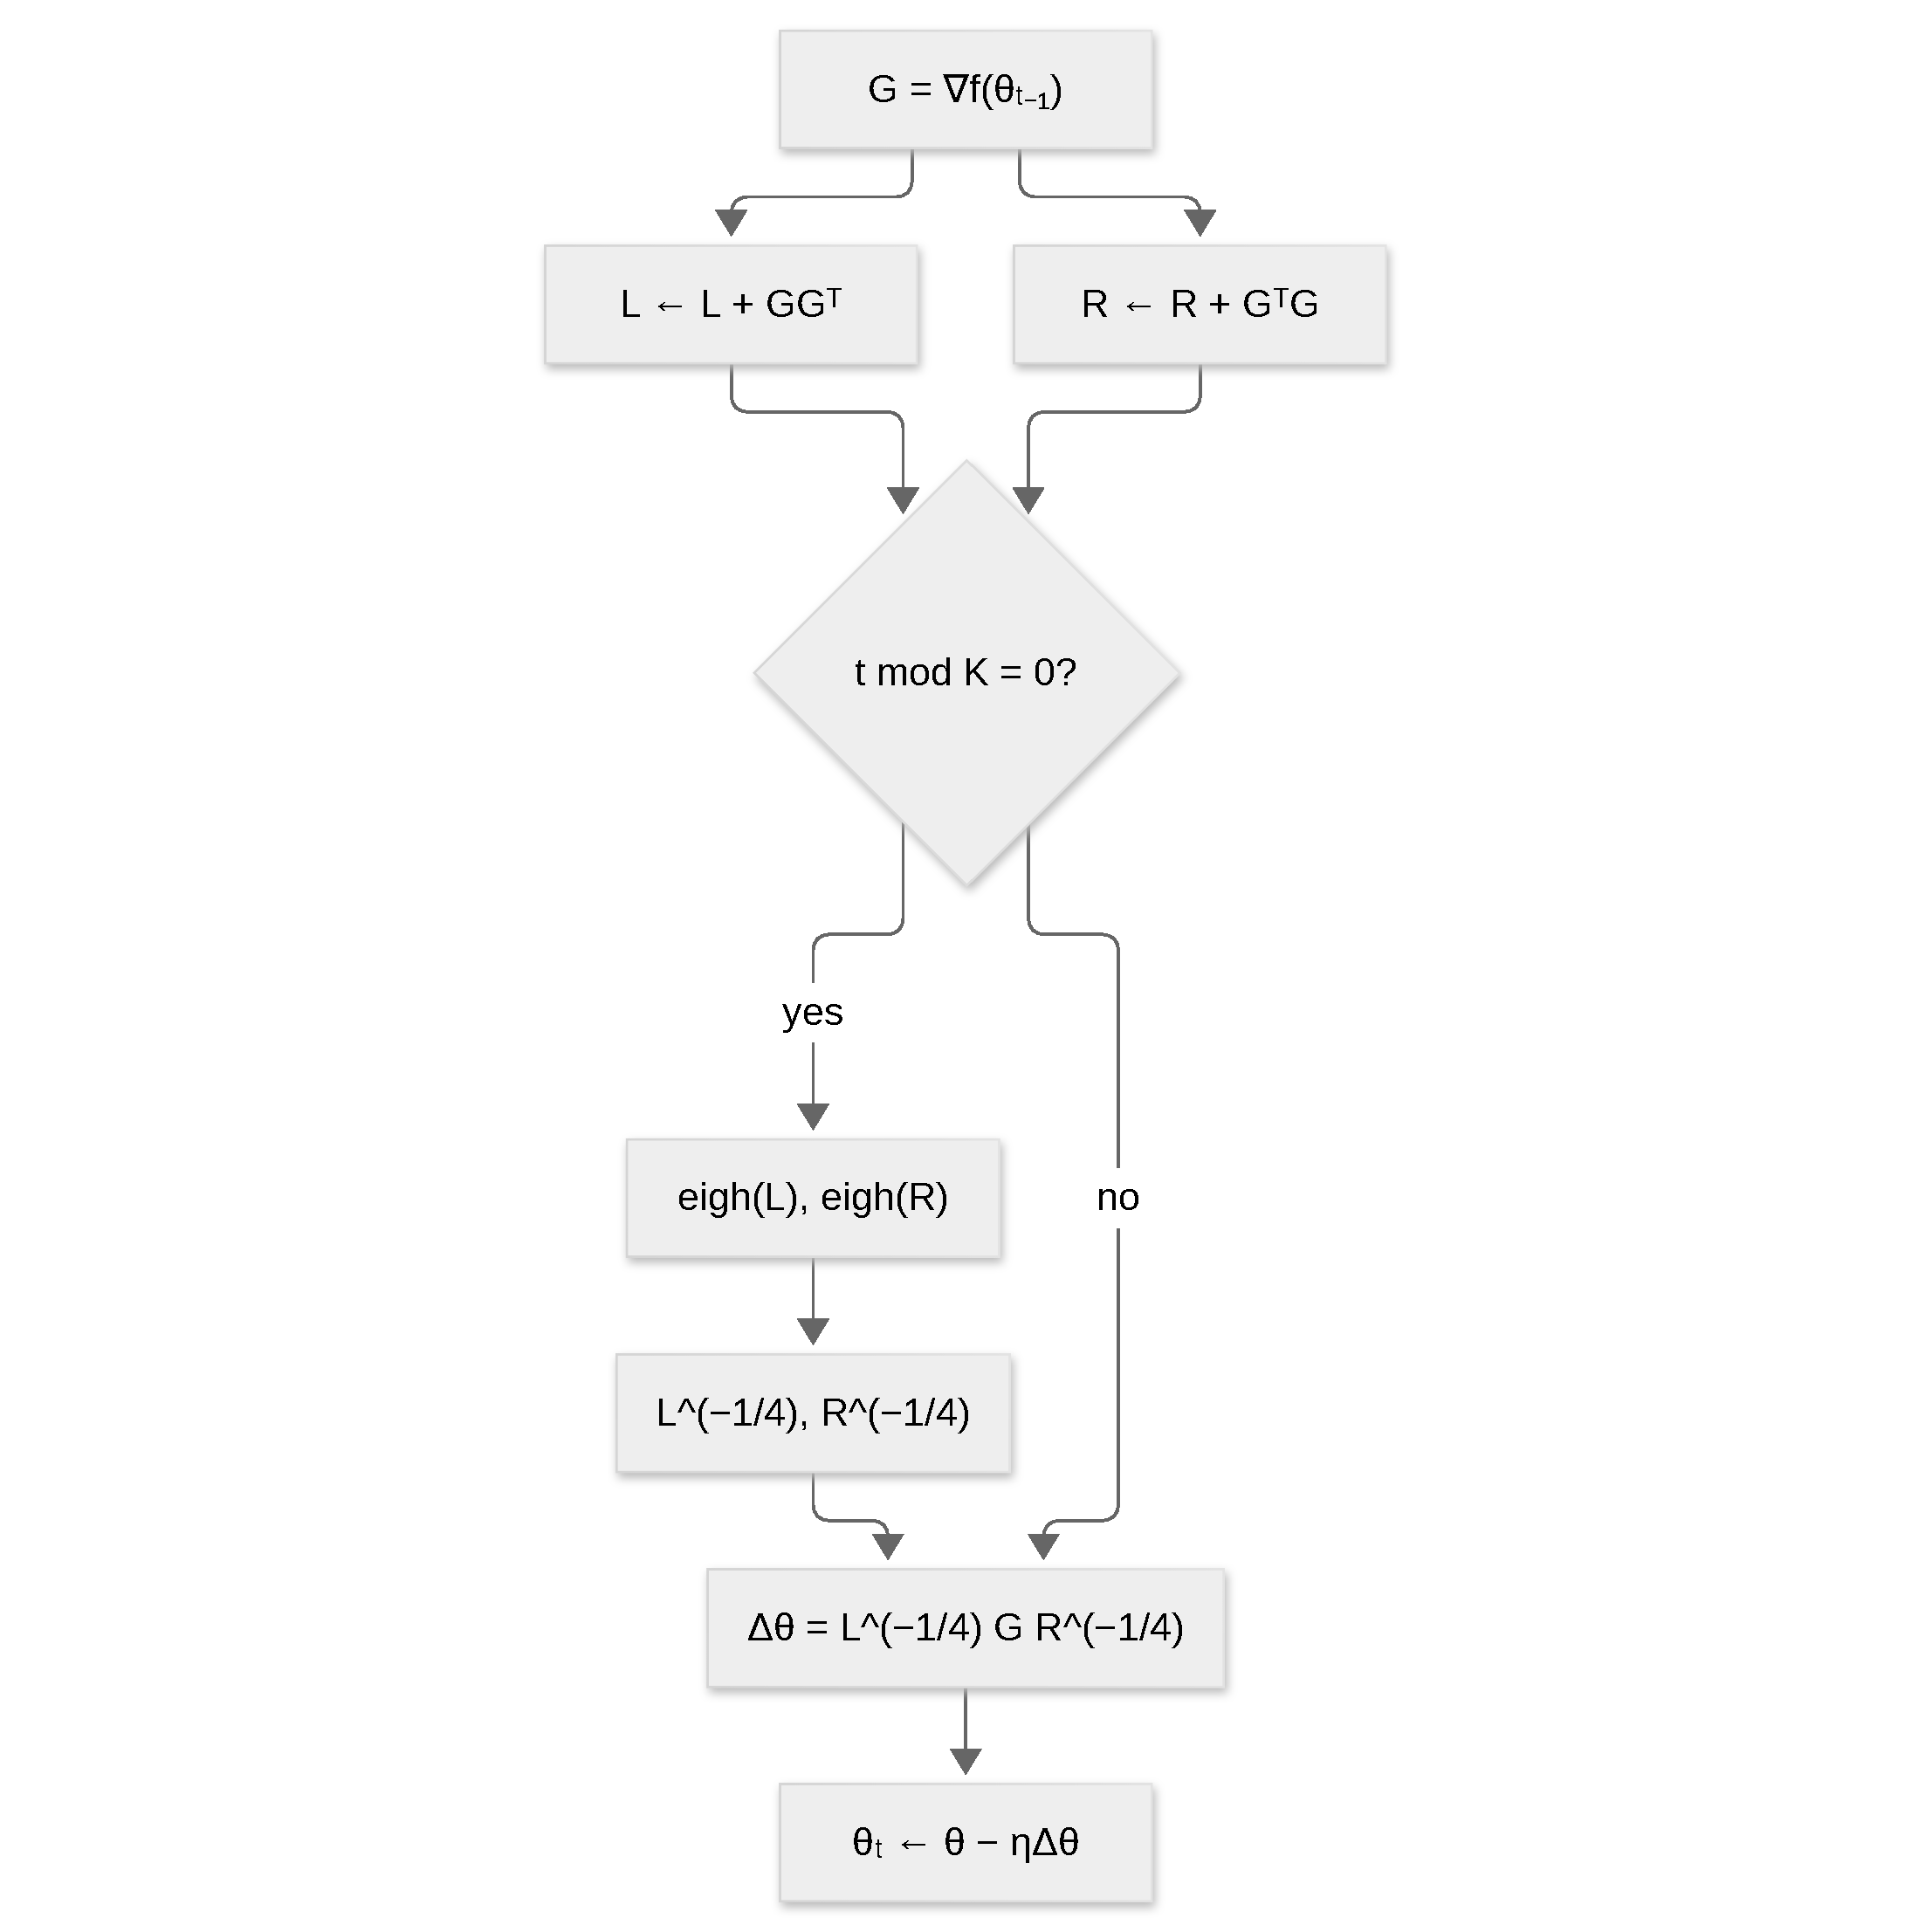
\includegraphics{../paper/figures/optimizers/shampoo.pdf}}
\caption{Flujo por paso de Shampoo: matrices de Gram factorizadas por Kronecker, eigendescomposición periódica y precondicionamiento del gradiente con raíz cuarta.}
\label{fig:opt-shampoo}
\end{figure}
Shampoo es un \textbf{método estructurado de segundo orden} que calcula precondicionadores matriciales a partir de estadísticas de producto exterior con estructura de Kronecker. Para una matriz de parámetros 2D $W \in \mathbb{R}^{m \times n}$:
\begin{align}
L_t &= L_{t-1} + G_t G_t^\top \quad\text{(matriz de Gram izquierda/filas, $m \times m$)} \\
R_t &= R_{t-1} + G_t^\top G_t \quad\text{(matriz de Gram derecha/columnas, $n \times n$)} \\
L_t^{-1/4} &= Q_L (\Lambda_L)^{-1/4} Q_L^\top \quad\text{(mediante eigendescomposición)} \\
R_t^{-1/4} &= Q_R (\Lambda_R)^{-1/4} Q_R^\top \\
\Delta W_t &= L_t^{-1/4} G_t R_t^{-1/4} \quad\text{(gradiente precondicionado)}
\end{align}
Shampoo aproxima el precondicionador de matriz completa de Adagrad $H^{-1/2}$ (donde $H$ es el Hessiano) utilizando estructura factorizada de Kronecker. En lugar de almacenar un precondicionador de $(mn) \times (mn)$, Shampoo mantiene dos matrices más pequeñas ($m \times m$ y $n \times n$), capturando correlaciones entre parámetros dentro y entre grupos. Las eigendescomposiciones se realizan periódicamente (e.g., cada $K=10$ pasos) para amortizar el costo.

\begin{algorithm}[H]
\caption{Shampoo (Precondicionamiento Matricial mediante Productos de Kronecker)}
\label{alg:shampoo}
\begin{algorithmic}[1]
\Require Parámetros iniciales $\theta_0$, tasa de aprendizaje $\eta$, intervalo de eigendescomposición $K$
\Ensure Parámetros actualizados $\theta_T$
\State Inicializar: $L \gets \epsilon I_m$, $R \gets \epsilon I_n$ (matrices de Gram izquierda y derecha)
\For{$t = 1, 2, \ldots, T$}
    \State $G \gets \nabla f(\theta_{t-1})$ \Comment{Gradiente}
    \State Actualizar matrices de Gram: $L \gets L + G G^\top$, $R \gets R + G^\top G$
    \If{$t \mod K == 0$}
        \State $Q_L, \Lambda_L \gets \text{eigh}(L)$ \Comment{Eigendescomposición de $L$}
        \State $Q_R, \Lambda_R \gets \text{eigh}(R)$ \Comment{Eigendescomposición de $R$}
        \State $L^{-1/4} \gets Q_L (\Lambda_L + \epsilon)^{-1/4} Q_L^\top$
        \State $R^{-1/4} \gets Q_R (\Lambda_R + \epsilon)^{-1/4} Q_R^\top$
    \EndIf
    \State $\Delta \theta \gets L^{-1/4} G R^{-1/4}$ \Comment{Gradiente precondicionado}
    \State $\theta_t \gets \theta_{t-1} - \eta \cdot \Delta \theta$
\EndFor
\Return $\theta_T$
\end{algorithmic}
\end{algorithm}

\paragraph{Contras.}
\begin{itemize}[leftmargin=*]
\item Eigendescomposiciones periódicas $O(m^3+n^3)$ y mayor cómputo por paso.
\item Asume estructura de parámetros 2D; los embeddings y sesgos requieren manejo aparte.
\end{itemize}

\paragraph{Ventajas.}
\begin{itemize}[leftmargin=*]
\item Precondicionamiento de segundo orden factorizado por Kronecker sin una matriz densa $(mn)\times(mn)$.
\item Demostrado efectivo a escala de producción y adecuado para matrices transformer de alto rango, con mejor condicionamiento y convergencia acelerada.
\end{itemize}

\paragraph{SOAP (Shampoo with Adam in eigenbasis).}
\begin{figure}[H]
\centering
\fitfigure{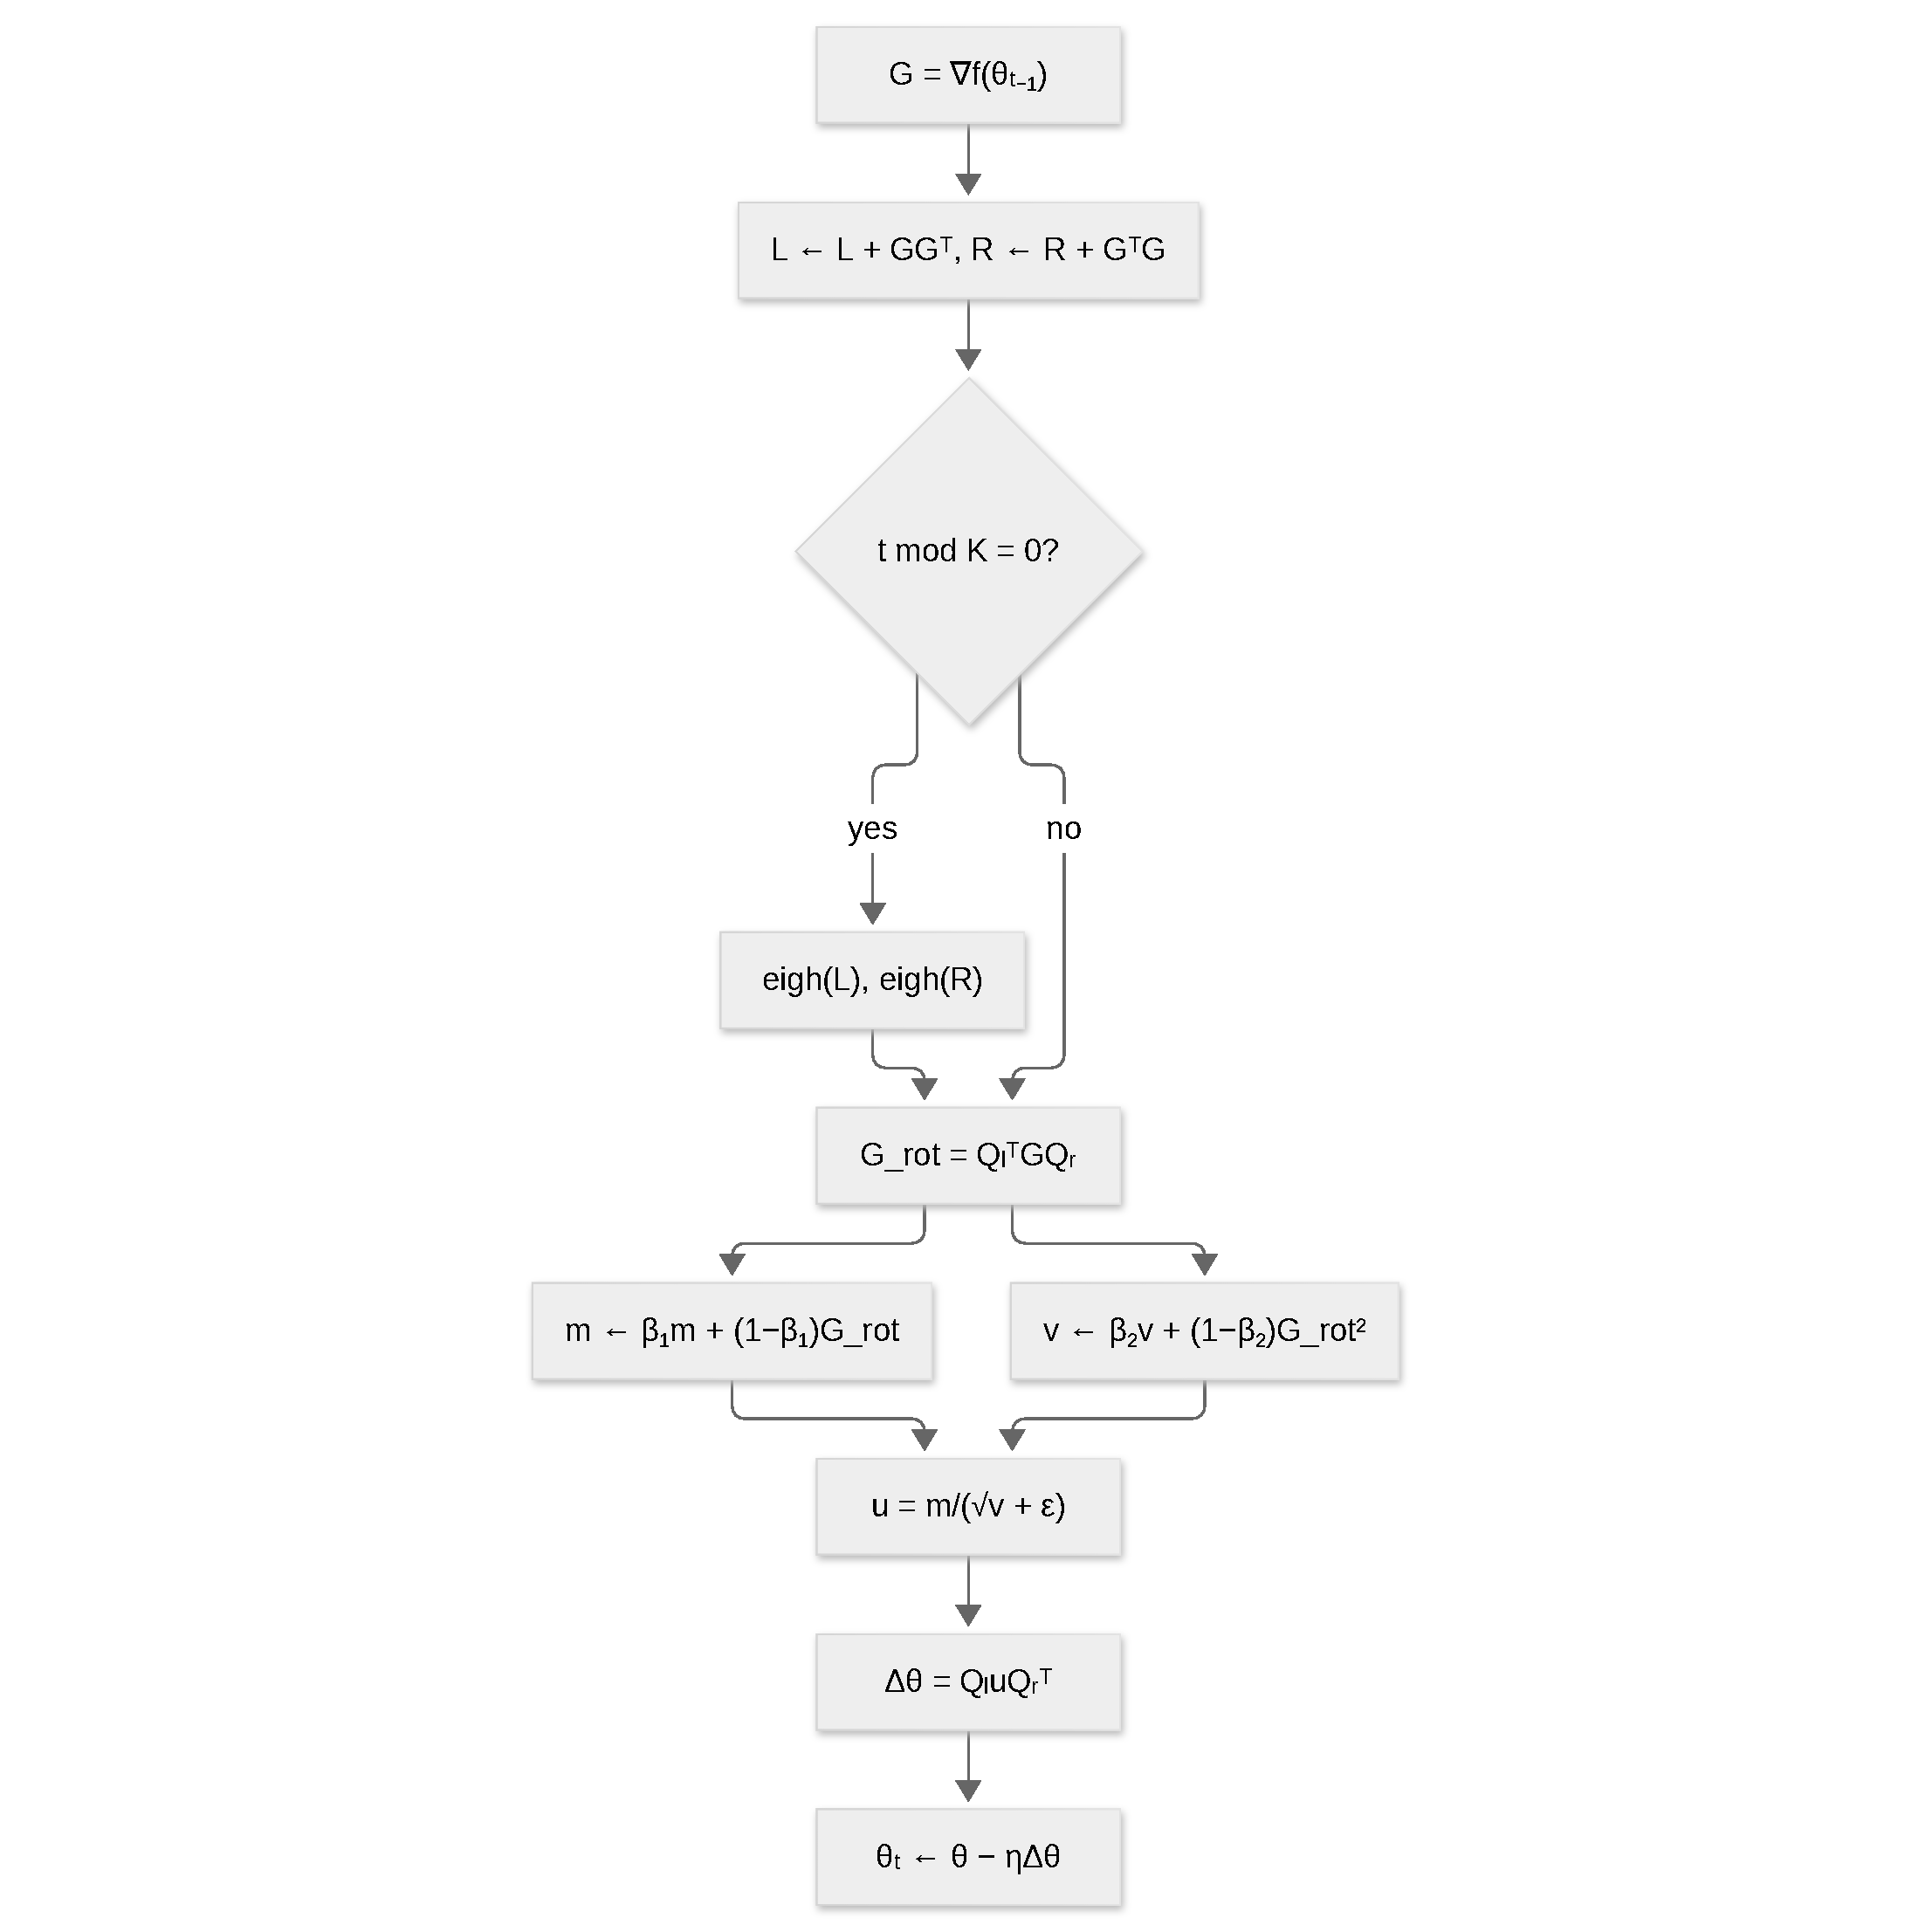
\includegraphics{../paper/figures/optimizers/soap.pdf}}
\caption{Flujo por paso de SOAP: momentos de Adam en la base de eigenvectores de Shampoo, rotados de vuelta al espacio de parámetros.}
\label{fig:opt-soap}
\end{figure}
SOAP es una variante simplificada de Shampoo que desacopla el precondicionamiento del seguimiento de momento. En lugar de álgebra matricial compleja sobre gradientes precondicionados, SOAP ejecuta Adam estándar en la base de eigenvectores de los precondicionadores de Shampoo:
\begin{align}
L_t &= L_{t-1} + G_t G_t^\top, \quad R_t = R_{t-1} + G_t^\top G_t \quad\text{(acumulación de Gram)} \\
Q_L, \Lambda_L &= \text{eigh}(L_t), \quad Q_R, \Lambda_R = \text{eigh}(R_t) \quad\text{(eigendescomposición periódica)} \\
G_t^{\text{rot}} &= Q_L^\top G_t Q_R \quad\text{(rotar gradiente a la base de eigenvectores)} \\
m_t^{\text{rot}} &= \beta_1 m_{t-1}^{\text{rot}} + (1-\beta_1) G_t^{\text{rot}} \\
v_t^{\text{rot}} &= \beta_2 v_{t-1}^{\text{rot}} + (1-\beta_2)(G_t^{\text{rot}})^2 \quad\text{(Adam en el espacio rotado)} \\
U_t^{\text{rot}} &= \frac{m_t^{\text{rot}}}{\sqrt{v_t^{\text{rot}}}+\epsilon}, \quad U_t = Q_L U_t^{\text{rot}} Q_R^\top \quad\text{(rotar de vuelta)}
\end{align}
La idea clave: todo el seguimiento de momento ocurre en la base de eigenvectores bien condicionada, simplificando la estabilidad numérica y el análisis teórico.

\begin{algorithm}[H]
\caption{SOAP (Shampoo with Adam in Eigenbasis)}
\label{alg:soap}
\begin{algorithmic}[1]
\Require Parámetros iniciales $\theta_0$, tasa de aprendizaje $\eta$, $\beta_1, \beta_2$, intervalo de eigendescomposición $K$
\Ensure Parámetros actualizados $\theta_T$
\State Inicializar: $L \gets \epsilon I_m$, $R \gets \epsilon I_n$, $m \gets 0$, $v \gets 0$
\For{$t = 1, 2, \ldots, T$}
    \State $G \gets \nabla f(\theta_{t-1})$ \Comment{Gradiente}
    \State Actualizar Gram: $L \gets L + G G^\top$, $R \gets R + G^\top G$
    \If{$t \mod K == 0$}
        \State $Q_L, \Lambda_L \gets \text{eigh}(L)$, $Q_R, \Lambda_R \gets \text{eigh}(R)$
    \EndIf
    \State $G^{\text{rot}} \gets Q_L^\top G Q_R$ \Comment{Rotar gradiente a la base de eigenvectores}
    \State $m \gets \beta_1 m + (1-\beta_1) G^{\text{rot}}$ \Comment{Media móvil exponencial (corregir sesgo externamente)}
    \State $v \gets \beta_2 v + (1-\beta_2) (G^{\text{rot}})^2$ \Comment{Segundo momento (corregir sesgo externamente)}
    \State $u \gets m / (\sqrt{v} + \epsilon)$ \Comment{Paso adaptativo en la base de eigenvectores}
    \State $\Delta \theta \gets Q_L u Q_R^\top$ \Comment{Rotar de vuelta al espacio de parámetros}
    \State $\theta_t \gets \theta_{t-1} - \eta \cdot \Delta \theta$
\EndFor
\Return $\theta_T$
\end{algorithmic}
\end{algorithm}

\paragraph{Contras.}
\begin{itemize}[leftmargin=*]
\item Hereda el costo de eigendescomposición periódica de Shampoo.
\item La rotación y la rotación inversa añaden multiplicaciones de matrices por paso.
\end{itemize}

\paragraph{Ventajas.}
\begin{itemize}[leftmargin=*]
\item Combina la estructura de curvatura explícita de Shampoo con la mecánica de momentum probada de Adam.
\item A menudo más limpio y estable que Shampoo completo, con eigendescomposiciones amortizadas cada $K$ pasos.
\end{itemize}

\paragraph{Lion (EvoLved Sign Momentum).}
\begin{figure}[H]
\centering
\fitfigure{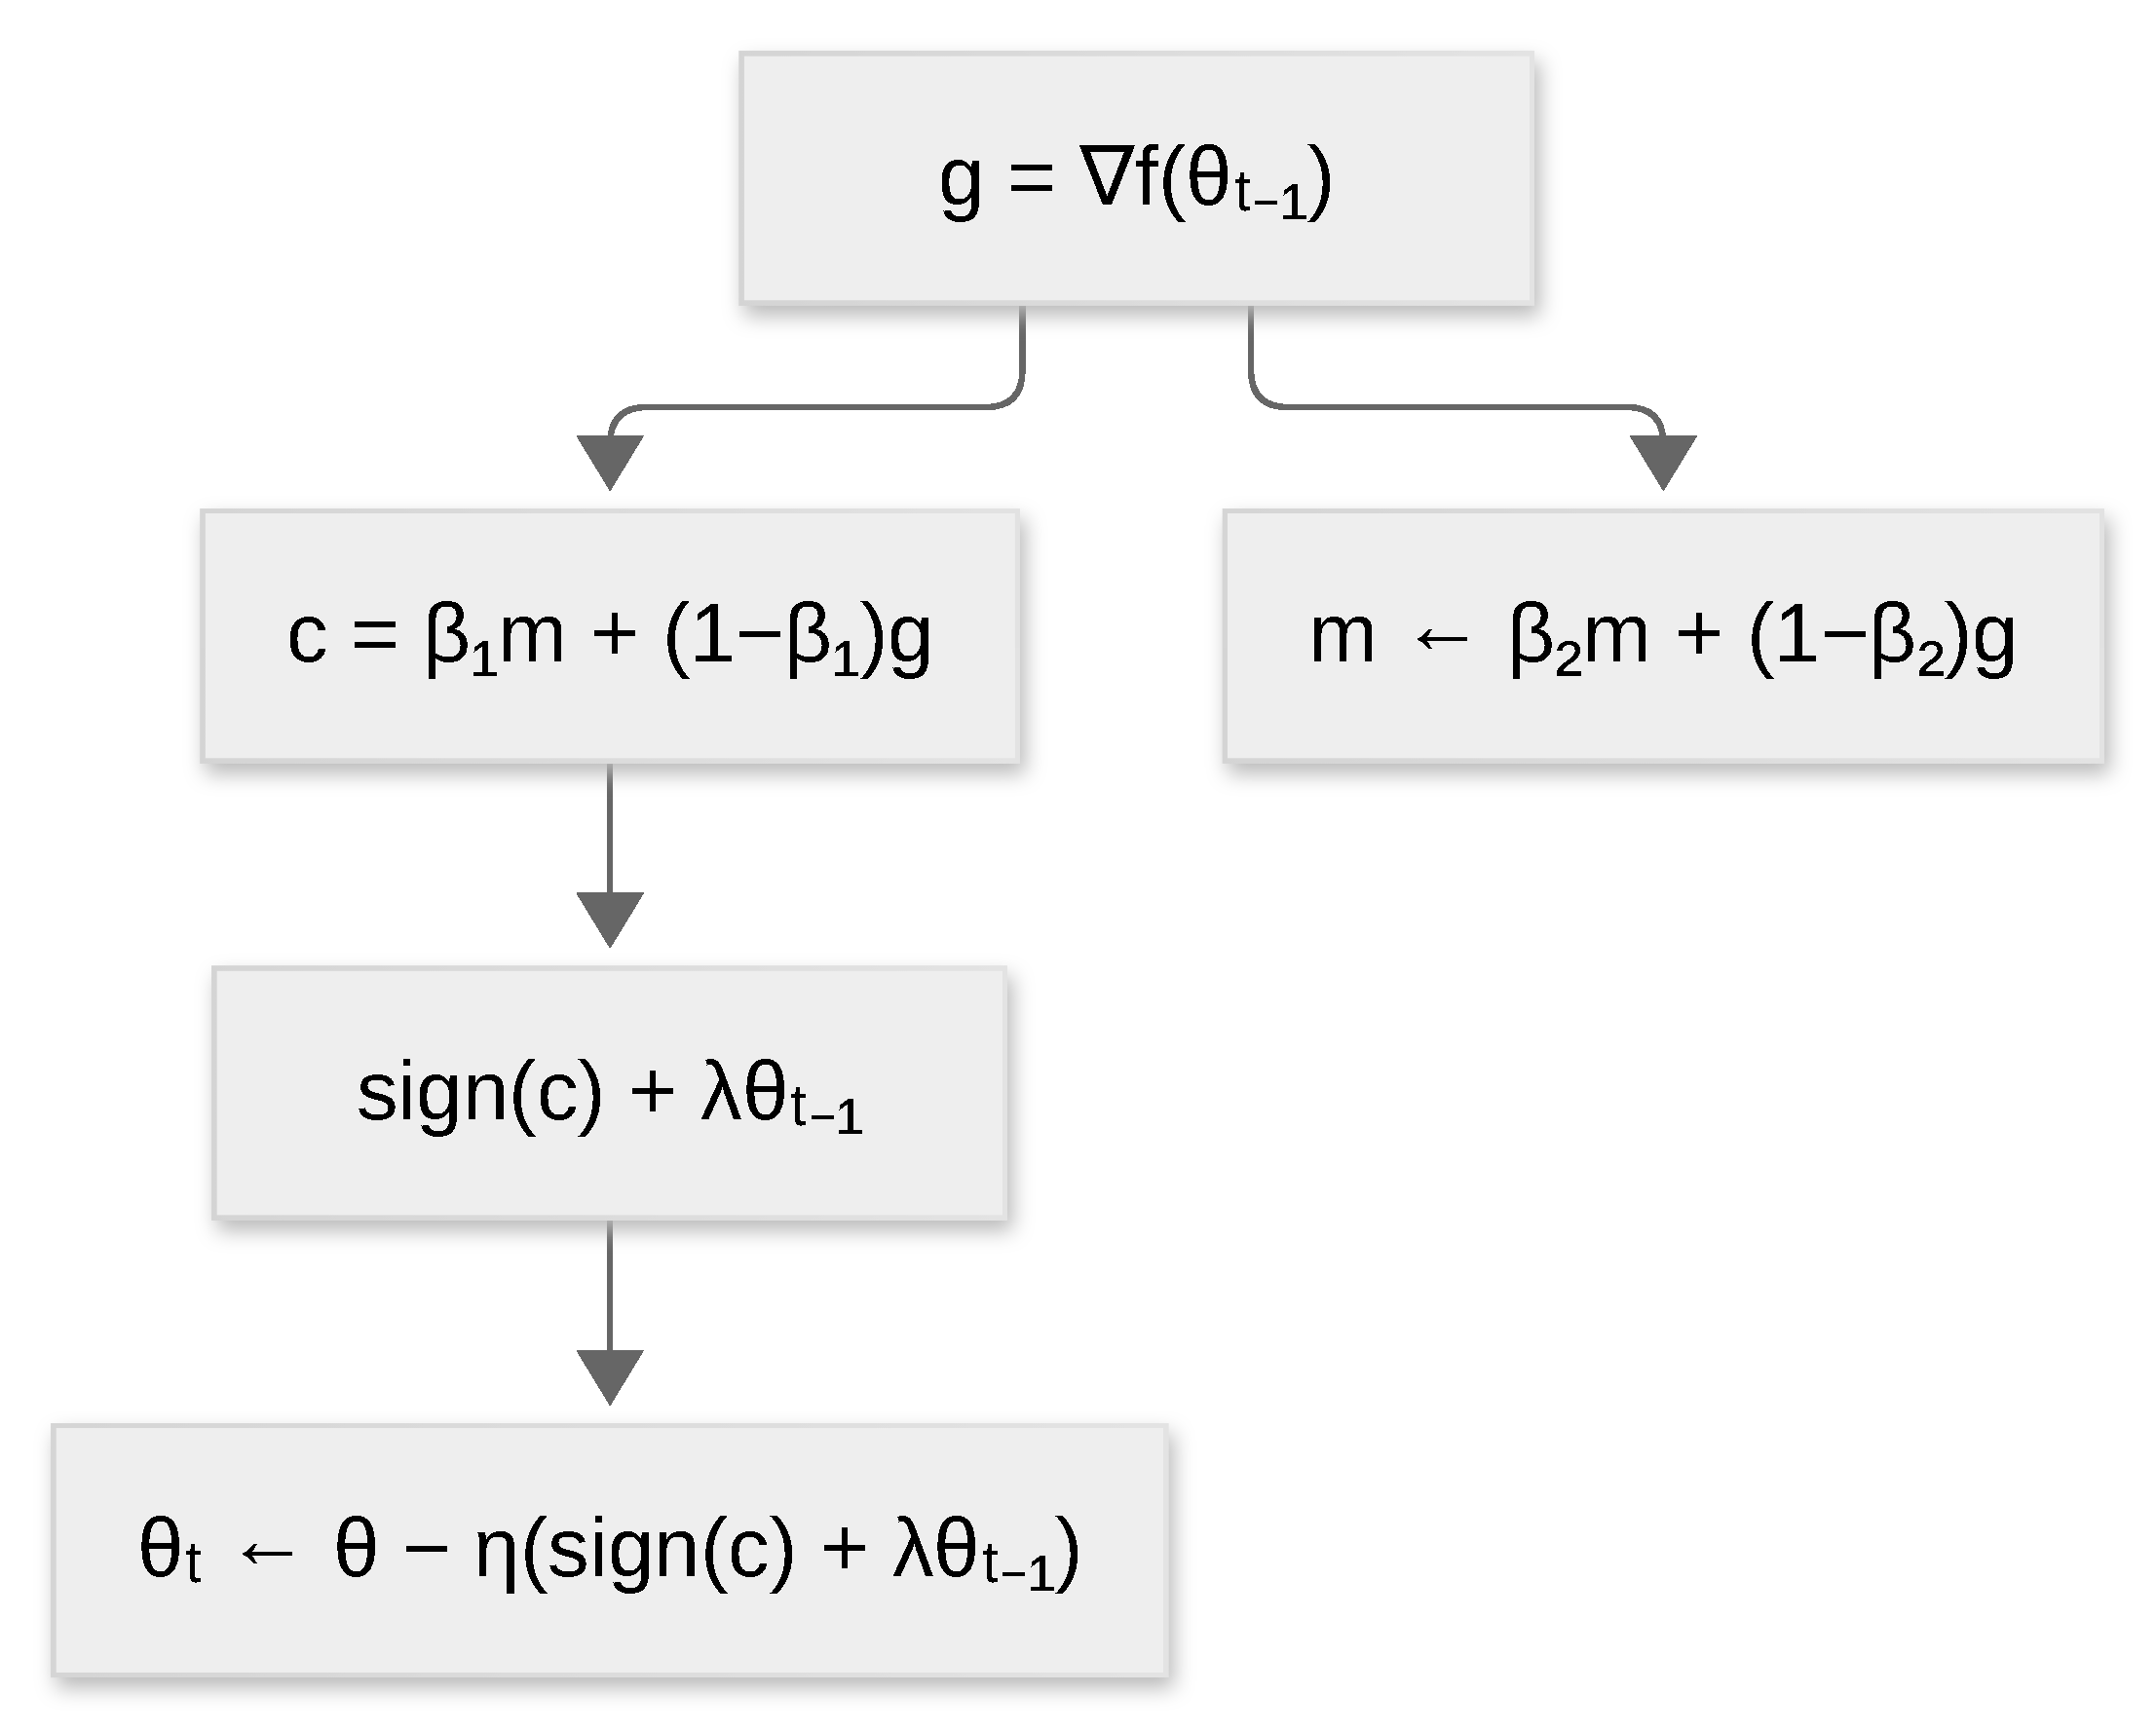
\includegraphics{../paper/figures/optimizers/lion.pdf}}
\caption{Flujo por paso de Lion: actualización por signo del momentum con acumulación de momentum desacoplada y decaimiento de pesos.}
\label{fig:opt-lion}
\end{figure}
Lion logra una \textbf{sobrecarga de memoria mínima} al usar actualizaciones basadas en signo en lugar de escalado adaptativo completo:
\begin{align}
c_t &= \beta_1 m_t + (1-\beta_1) g_t \quad\text{(entrada de momento)} \\
\theta_{t+1} &= \theta_t - \eta \left(\text{sign}(c_t) + \lambda\theta_t\right) \quad\text{(actualización con operador signo)} \\
m_{t+1} &= \beta_2 m_t + (1-\beta_2) g_t \quad\text{(acumulación de momento)}
\end{align}
Todas las operaciones de escalado elemento a elemento se reemplazan con \texttt{sign()}, que produce $\{-1, 0, +1\}$. Esto reduce drásticamente la memoria en comparación con métodos tipo Adam: Lion almacena solo el búfer de momento, sin varianza de segundo momento.

\begin{algorithm}[H]
\caption{Lion (EvoLved Sign Momentum)}
\label{alg:lion}
\begin{algorithmic}[1]
\Require Parámetros iniciales $\theta_0$, tasa de aprendizaje $\eta$, $\beta_1, \beta_2$, decaimiento de pesos $\lambda$
\Ensure Parámetros actualizados $\theta_T$
\State Inicializar: $m \gets 0$ (búfer de momento)
\For{$t = 1, 2, \ldots, T$}
    \State $g \gets \nabla f(\theta_{t-1})$ \Comment{Gradiente}
    \State $c \gets \beta_1 m + (1-\beta_1) g$ \Comment{Entrada de momento}
    \State $\theta_t \gets \theta_{t-1} - \eta (\text{sign}(c) + \lambda \theta_{t-1})$ \Comment{Actualización basada en signo con decaimiento de pesos}
    \State $m \gets \beta_2 m + (1-\beta_2) g$ \Comment{Acumulación de momento (desacoplada)}
\EndFor
\Return $\theta_T$
\end{algorithmic}
\end{algorithm}

\paragraph{Contras.}
\begin{itemize}[leftmargin=*]
\item Las actualizaciones por signo sacrifican la adaptación elemento a elemento de la tasa de aprendizaje que hace efectivo a Adam.
\item Puede ser menos robusto que los métodos de la familia Adam en tareas que requieren escalado adaptativo.
\end{itemize}

\paragraph{Ventajas.}
\begin{itemize}[leftmargin=*]
\item Almacena solo el búfer de momentum, sin varianza de segundo momento.
\item Opción de alto rendimiento y baja memoria para regímenes de lotes grandes donde domina la memoria de activaciones.
\end{itemize}

\paragraph{Sophia (Second-Order Hessian Information with Optimized Approximation).}
\begin{figure}[H]
\centering
\fitfigure{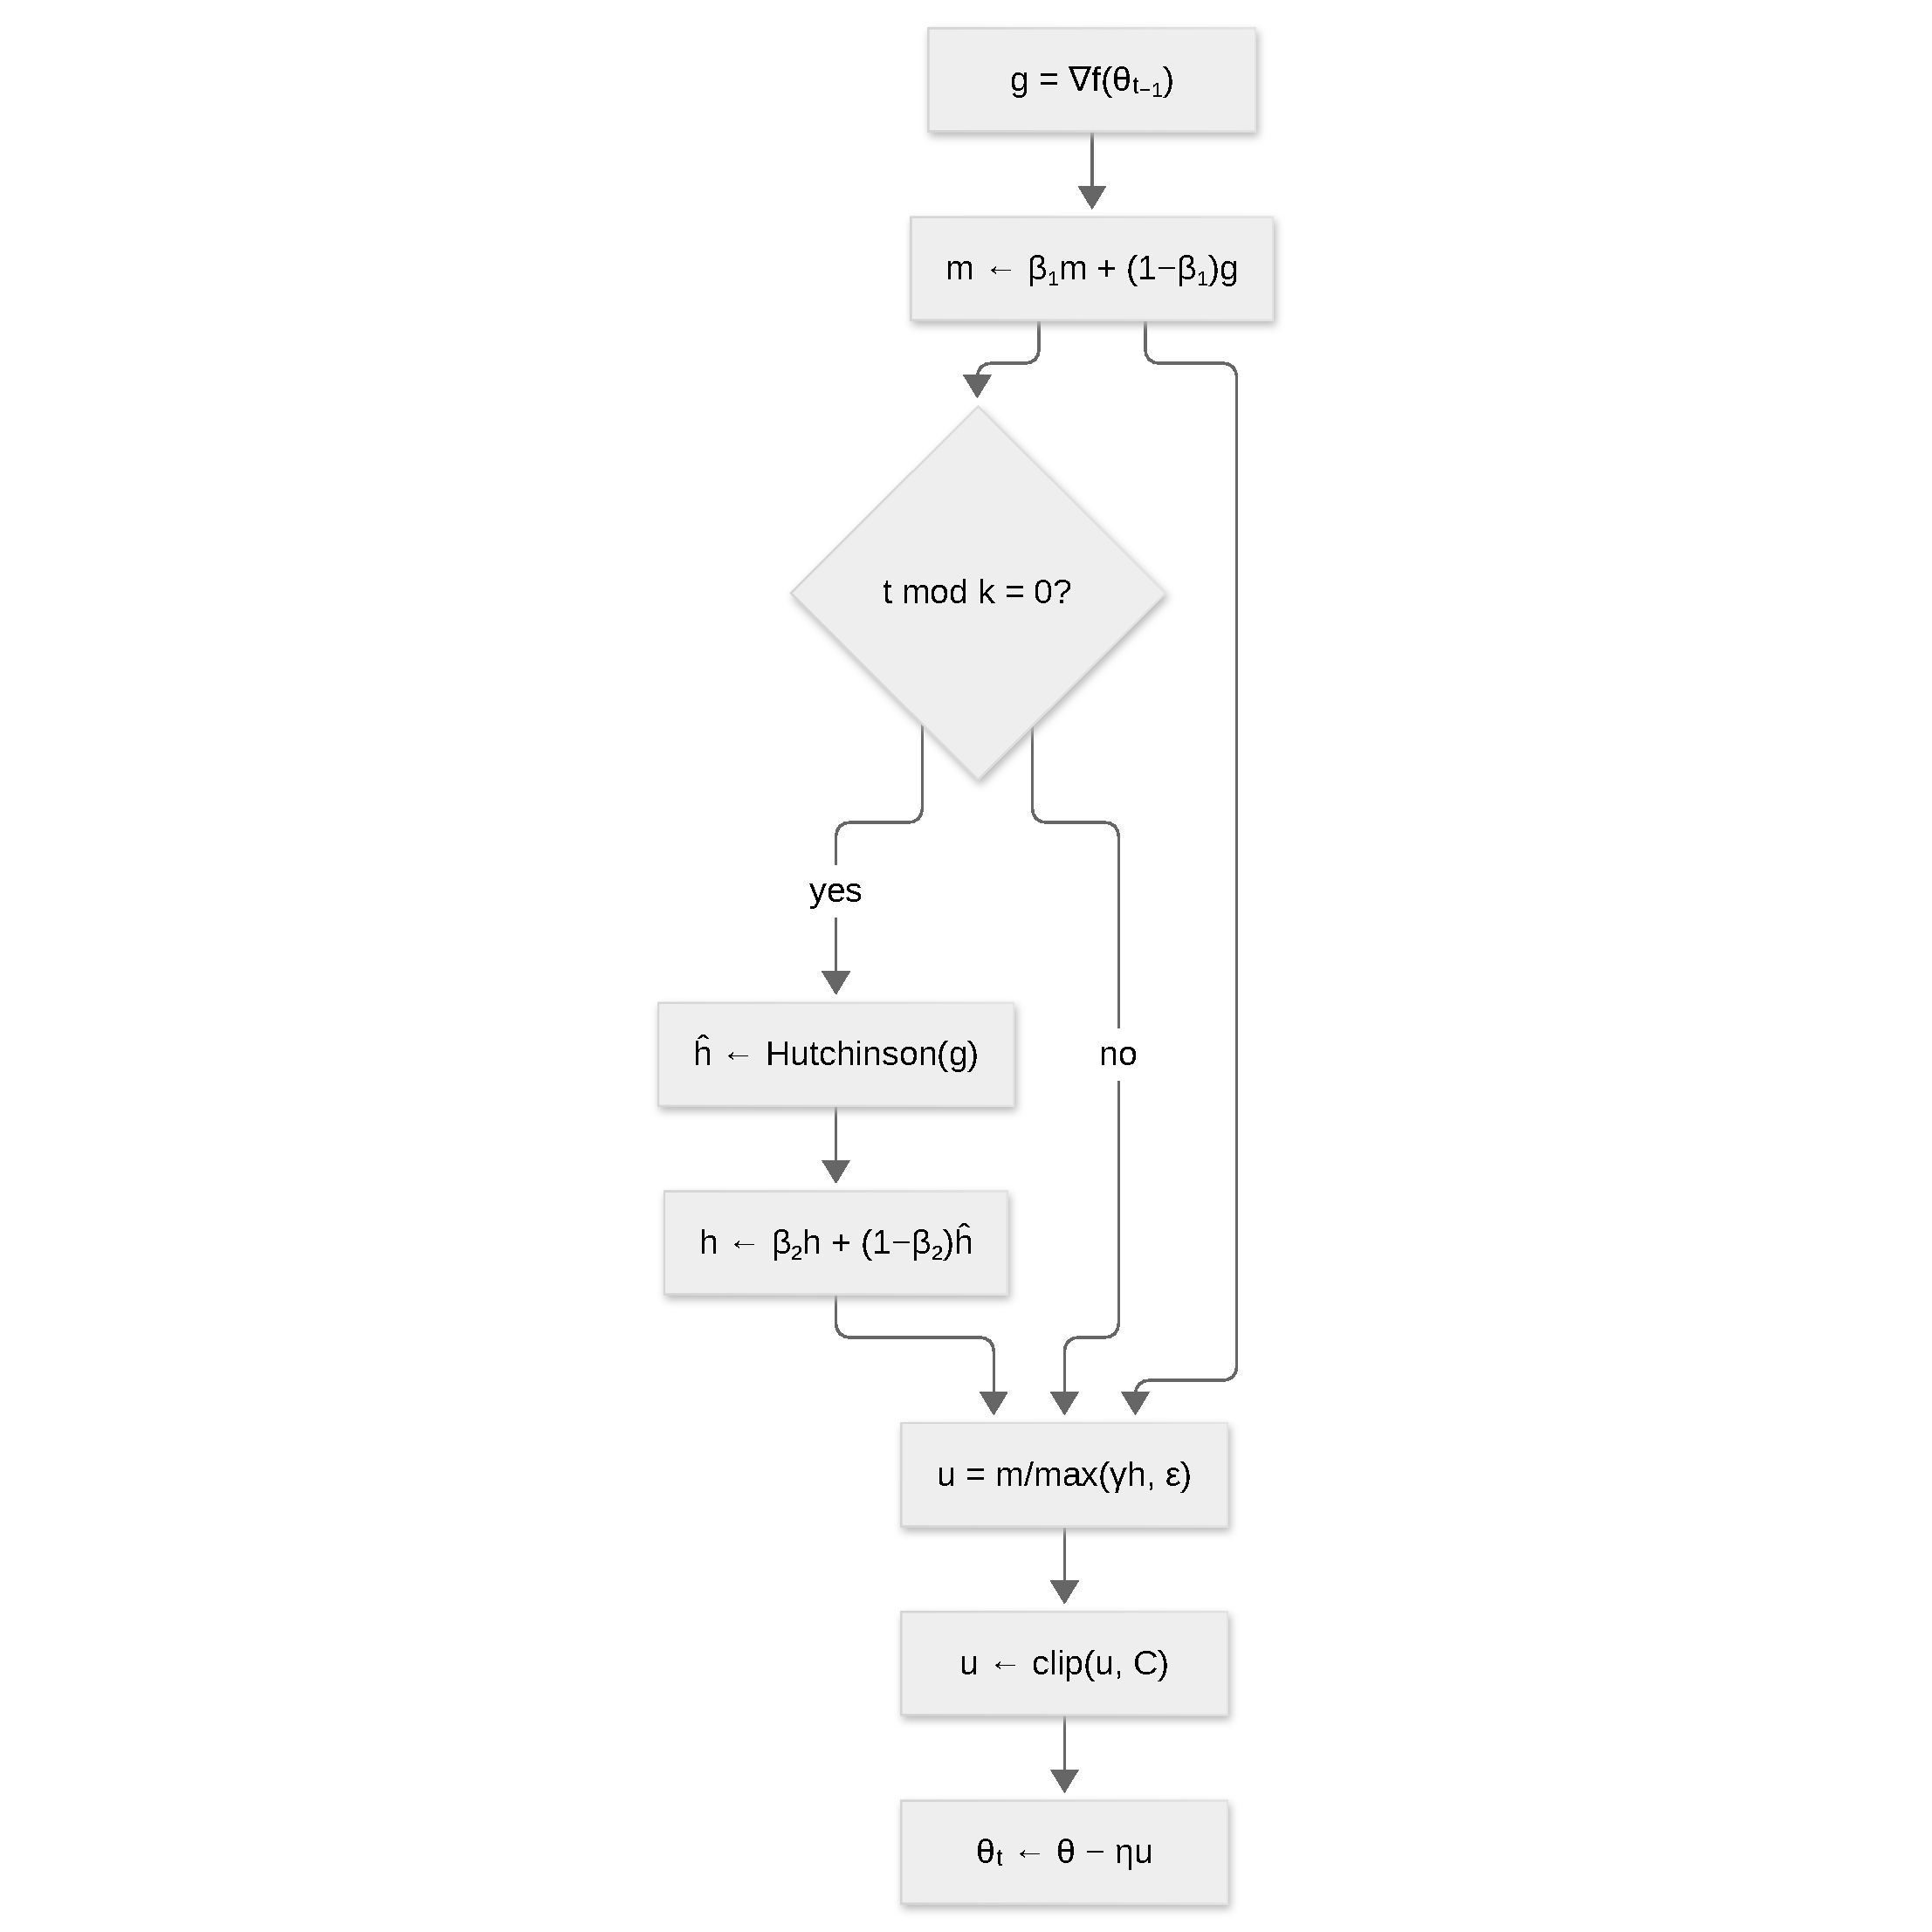
\includegraphics{../paper/figures/optimizers/sophia.pdf}}
\caption{Flujo por paso de Sophia: estimación diagonal del Hessiano mediante Hutchinson con pasos recortados conscientes de la curvatura.}
\label{fig:opt-sophia}
\end{figure}
Sophia utiliza \textbf{estimaciones diagonales del Hessiano} para escalado consciente de la curvatura sin el costo de memoria y cómputo de los métodos densos de segundo orden.
\begin{align}
m_t &= \beta_1 m_{t-1} + (1-\beta_1) g_t \quad\text{(momento de primer orden)} \\
h_t &= \beta_2 h_{t-(k-1)} + (1-\beta_2) \hat{h}_t \quad\text{(Hessiano diagonal, actualizado cada $k$ pasos)} \\
\text{clip}(x, C) &= \min(\max(x, -C), C) \quad\text{(recorte elemento a elemento)} \\
\theta_{t+1} &= \theta_t - \eta \cdot \text{clip}\left(\frac{m_t}{\max(\gamma h_t, \epsilon)}, 1\right)
\end{align}
donde $\hat{h}_t$ es una estimación diagonal (e.g., estimador de traza de Hutchinson) y $\gamma$ es un factor de escala. El Hessiano diagonal $h_t$ captura la curvatura local, permitiendo que el optimizador tome pasos más pequeños en direcciones pronunciadas y pasos más grandes en direcciones planas. La operación de recorte $\text{clip}(\cdot, 1)$ evita que los pasos adaptativos exploten.

\begin{algorithm}[H]
\caption{Sophia (Hessiano Diagonal con Actualizaciones Recortadas)}
\label{alg:sophia}
\begin{algorithmic}[1]
\Require Parámetros iniciales $\theta_0$, tasa de aprendizaje $\eta$, $\beta_1, \beta_2$, frecuencia de actualización del Hessiano $k$, umbral de recorte $C$
\Ensure Parámetros actualizados $\theta_T$
\State Inicializar: $m \gets 0$, $h \gets \epsilon$ (estimación diagonal del Hessiano)
\For{$t = 1, 2, \ldots, T$}
    \State $g \gets \nabla f(\theta_{t-1})$
    \State $m \gets \beta_1 m + (1-\beta_1) g$ \Comment{Momento de primer orden (corregir sesgo externamente)}
    \If{$t \mod k == 0$}
        \State $\hat{h} \gets \text{HutchinsonEstimate}(g)$ \Comment{Hessiano diagonal mediante Hutchinson}
        \State $h \gets \beta_2 h + (1-\beta_2) \hat{h}$ \Comment{Actualizar estimación del Hessiano}
    \EndIf
    \State $u \gets \frac{m}{\max(\gamma h, \epsilon)}$ \Comment{Paso adaptativo (elemento a elemento)}
    \State $u \gets \text{clip}(u, C)$ \Comment{Recorte elemento a elemento a $[-C, C]$}
    \State $\theta_t \gets \theta_{t-1} - \eta \cdot u$
\EndFor
\Return $\theta_T$
\end{algorithmic}
\end{algorithm}

\paragraph{Contras.}
\begin{itemize}[leftmargin=*]
\item Las estimaciones de Hutchinson añaden cómputo periódico y ruido a la señal de curvatura.
\item La estimación del Hessiano puede quedar desactualizada entre refrescos.
\end{itemize}

\paragraph{Ventajas.}
\begin{itemize}[leftmargin=*]
\item Escalado consciente de la curvatura sin el costo $O(n^2)$ u $O(n^3)$ de los métodos completos de segundo orden.
\item Los pasos recortados evitan explosiones y funcionan particularmente bien en el ajuste fino de segunda pasada.
\end{itemize}

\paragraph{Muon (Ortogonalización de Newton-Schulz).}
\begin{figure}[H]
\centering
\fitfigure{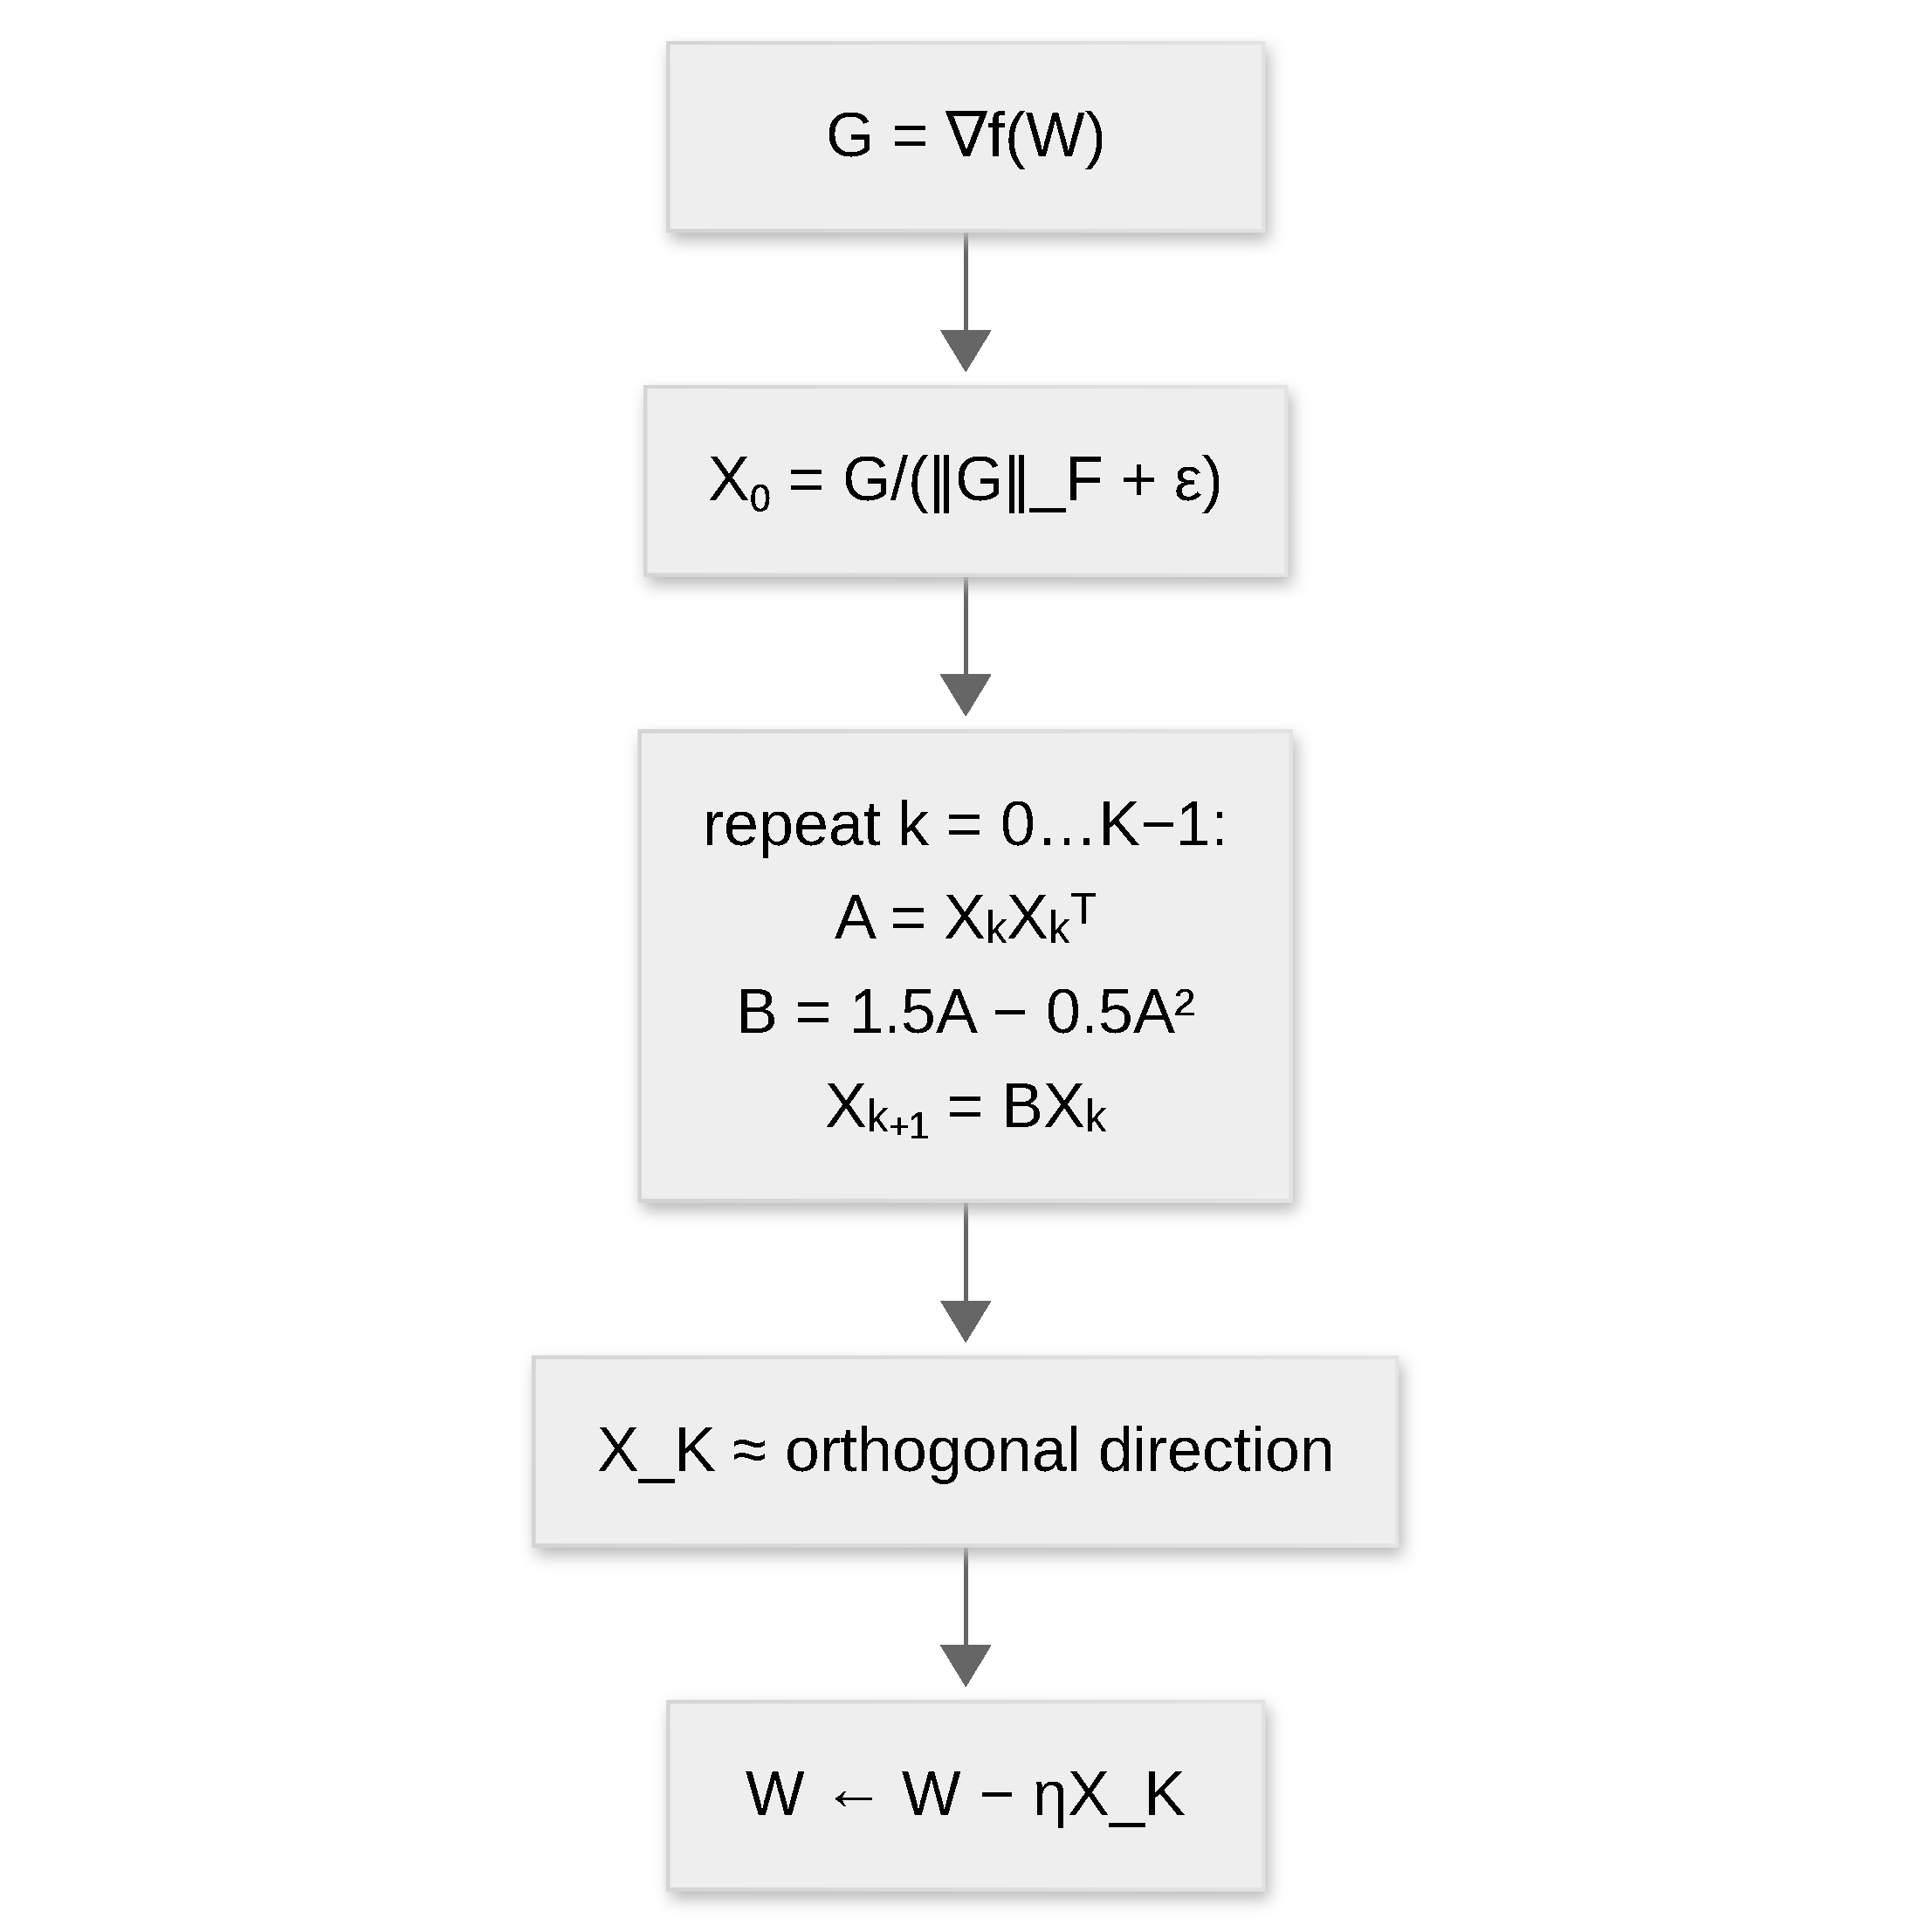
\includegraphics{../paper/figures/optimizers/muon.pdf}}
\caption{Flujo por paso de Muon: normalización de Frobenius seguida de iteraciones de Newton-Schulz que ortogonalizan la dirección de actualización.}
\label{fig:opt-muon}
\end{figure}
Muon es un \textbf{optimizador orientado a la ortogonalidad} que reformula la geometría de actualización utilizando iteraciones polinomiales de Newton-Schulz para ortogonalización. Para una matriz de parámetros 2D $W$ con gradiente $G_t$:
\begin{align}
X_0 &= \frac{G_t}{\|G_t\|_F + \epsilon} \quad\text{(gradiente normalizado)} \\
A_k &= X_k X_k^\top \quad\text{(Gramiana)} \\
B_k &= b A_k + c A_k^2 \quad\text{(paso polinomial, coeficientes $b, c$ de Newton-Schulz)} \\
X_{k+1} &= a X_k + B_k X_k \quad\text{(iteración $k=0,1,\ldots,4$)} \\
W_{t+1} &= W_t - \eta X_K \quad\text{(actualización con dirección ortogonalizada)}
\end{align}
Muon realiza 5 iteraciones de Newton-Schulz para producir una dirección aproximadamente ortogonal, asegurando que las actualizaciones respeten restricciones geométricas. La justificación: las actualizaciones ortogonales preservan las normas durante el entrenamiento, evitando la deriva de norma observada en métodos basados en momento.

Siguiendo la receta híbrida de \citet{shen_convergence_2025}, la actualización ortogonalizada se reserva para las matrices de pesos de capas ocultas (grupos $\mathtt{attention}$, $\mathtt{ffn}$ y otros bloques ocultos). Las tablas de embeddings, los encodings posicionales aprendidos, los heads de salida y todo parámetro no matricial (sesgos, escalas de normalización, kernels de convolución) se entrenan con AdamW desacoplado en lugar de omitirse, usando los valores por grupo de tasa de aprendizaje, weight decay, $\beta_1, \beta_2$ y $\epsilon$ de la configuración.

\begin{algorithm}[H]
\caption{Muon (Ortogonalización de Newton-Schulz)}
\label{alg:muon}
\begin{algorithmic}[1]
\Require Parámetros iniciales $\theta$, tasa de aprendizaje $\eta$, iteraciones Newton-Schulz $K$
\Ensure Parámetros actualizados $\theta_T$
\For{cada parámetro $P$}
    \If{$P$ es una matriz 2D de capa oculta $W$}
        \State $G \gets \nabla f(W)$ \Comment{Gradiente}
        \State $X_0 \gets \frac{G}{\|G\|_F + \epsilon}$ \Comment{Normalizar gradiente por norma de Frobenius}
        \For{$k = 0, 1, \ldots, K-1$}
            \State $A_k \gets X_k X_k^\top$ \Comment{Gramiana (costo: $O(mn^2)$ o $O(m^2n)$ para matrices altas/anchas)}
            \State $B_k \gets (3/2) A_k - (1/2) A_k^2$ \Comment{Coeficientes de Newton-Schulz}
            \State $X_{k+1} \gets B_k X_k$ \Comment{Paso polinomial}
        \EndFor
        \State $W \gets W - \eta X_K$ \Comment{Actualizar con dirección ortogonalizada}
    \Else
        \State $P \gets \operatorname{AdamW}(P, \nabla f(P); \eta, \beta_1, \beta_2, \epsilon, \lambda)$ \Comment{Respaldo híbrido: embeddings, pos, heads, no matriciales}
    \EndIf
\EndFor
\Return $\theta_T$
\end{algorithmic}
\end{algorithm}

\paragraph{Contras.}
\begin{itemize}[leftmargin=*]
\item Varias multiplicaciones de matrices por iteración de Newton-Schulz; se requieren kernels personalizados eficientes.
\item La construcción ortogonalizada está definida solo para matrices 2D; las clases de parámetros restantes dependen del respaldo AdamW y de su calibración de tasa de aprendizaje por grupo.
\end{itemize}

\paragraph{Ventajas.}
\begin{itemize}[leftmargin=*]
\item Las actualizaciones ortogonalizadas preservan las normas y evitan la deriva de norma de los métodos basados en momento.
\item Resultados prometedores en entrenamiento a gran escala con una geometría de actualización fundamentalmente mejor condicionada.
\end{itemize}

\paragraph{Turbo-Muon (Ortogonalización Precondicionada con AOL).}
\begin{figure}[H]
\centering
\fitfigure{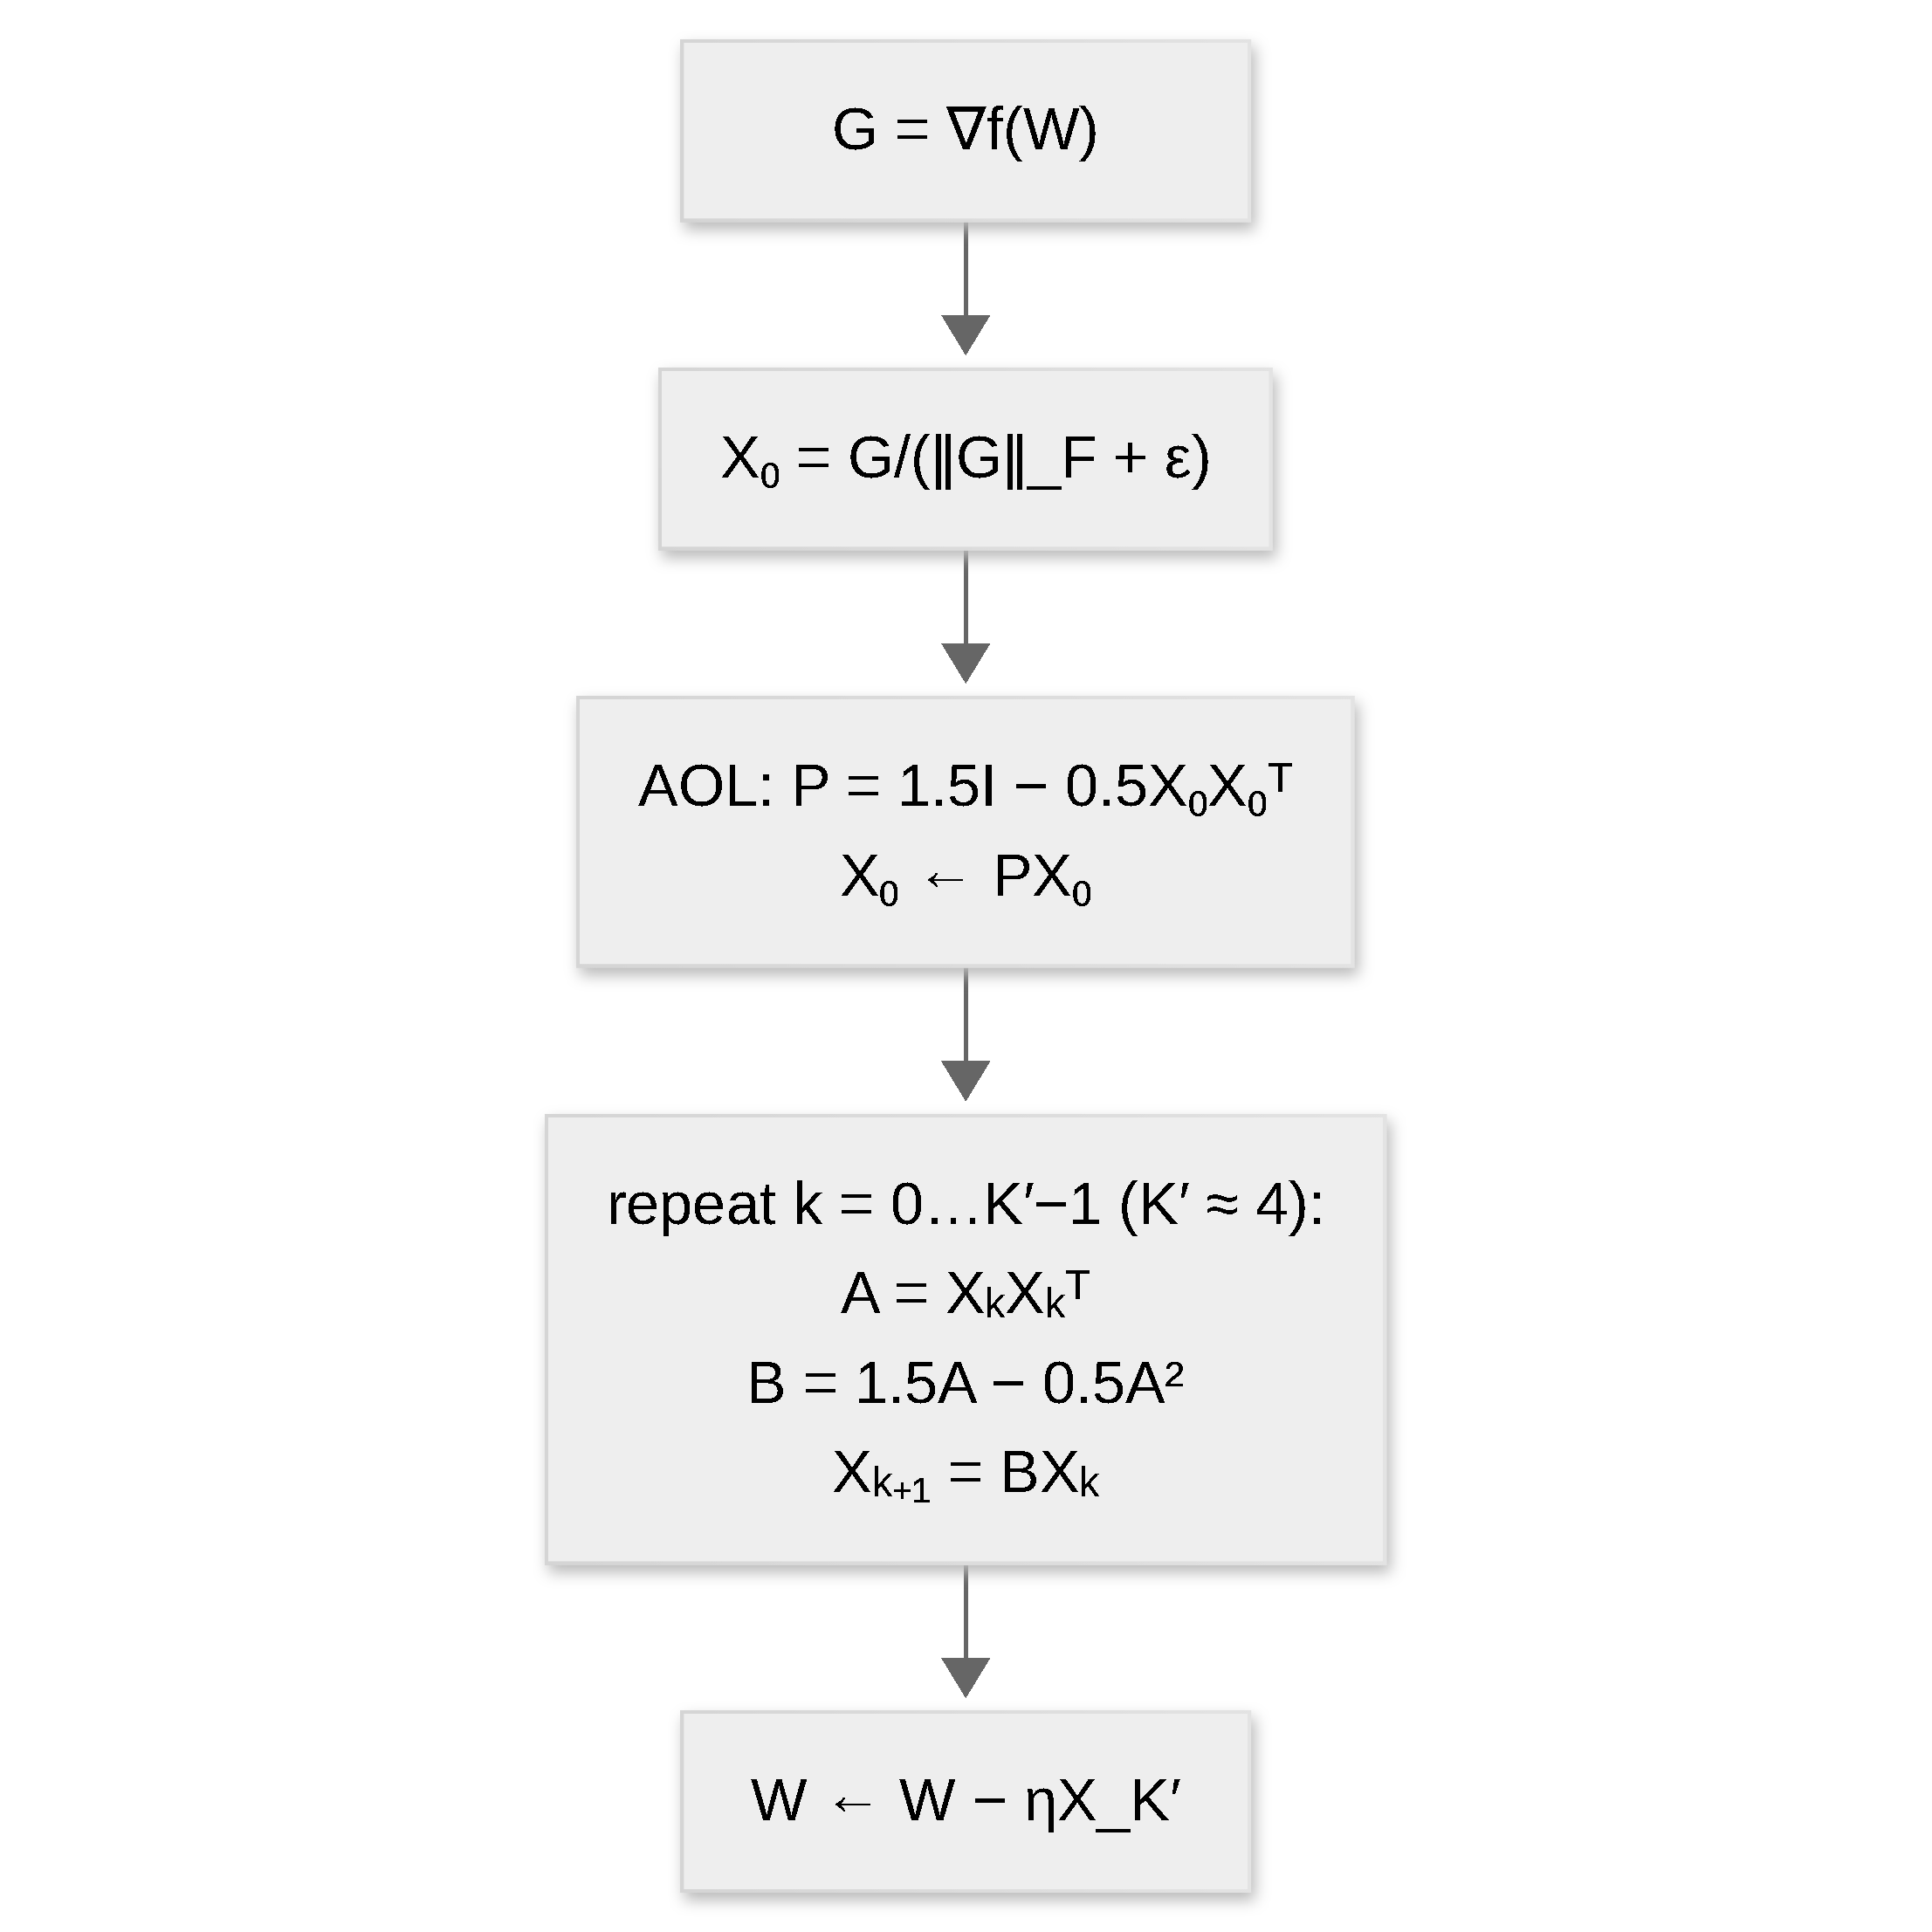
\includegraphics{../paper/figures/optimizers/turbo-muon.pdf}}
\caption{Flujo por paso de Turbo-Muon: precondicionamiento casi ortogonal (AOL) antes de las iteraciones de Newton-Schulz, reduciendo su número.}
\label{fig:opt-turbo-muon}
\end{figure}
Turbo-Muon añade un paso de \textbf{precondicionamiento casi-ortogonal} (AOL) antes de las iteraciones de Newton-Schulz. El precondicionador $P = 1.5I - 0.5X_0X_0^\top$ se aplica al gradiente normalizado, reduciendo el número de pasos de ortogonalización requeridos a cuatro mientras preserva la geometría de actualización ortogonalizada. Hereda el enrutamiento híbrido de Muon: solo se ortogonalizan las matrices 2D de capas ocultas, mientras que las tablas de embeddings, los encodings posicionales aprendidos, los heads de salida y los parámetros no matriciales reciben actualizaciones AdamW desacopladas.

\begin{algorithm}[H]
\caption{Turbo-Muon (Ortogonalización Precondicionada con AOL)}
\label{alg:turbo-muon}
\begin{algorithmic}[1]
\Require Parámetros iniciales $\theta$, tasa de aprendizaje $\eta$, iteraciones Newton-Schulz $K'$ (típicamente 4)
\Ensure Parámetros actualizados $\theta_T$
\For{cada parámetro $P$}
    \If{$P$ es una matriz 2D de capa oculta $W$}
        \State $G \gets \nabla f(W)$ \Comment{Gradiente}
        \State $X_0 \gets \frac{G}{\|G\|_F + \epsilon}$ \Comment{Normalizar gradiente}
        \State \textbf{AOL (Almost-Orthogonal preconditioner):} \Comment{Paso de precondicionamiento}
        \State $P \gets (1.5 I - 0.5 X_0 X_0^\top)$ \Comment{Matriz de precondicionamiento}
        \State $X_0 \gets P X_0$ \Comment{Inicio precondicionado}
        \For{$k = 0, 1, \ldots, K'-1$}
            \State $A_k \gets X_k X_k^\top$
            \State $B_k \gets (3/2) A_k - (1/2) A_k^2$
            \State $X_{k+1} \gets B_k X_k$ \Comment{Iteraciones reducidas gracias al precondicionamiento AOL}
        \EndFor
        \State $W \gets W - \eta X_{K'}$ \Comment{Actualizar con dirección ortogonalizada precondicionada}
    \Else
        \State $P \gets \operatorname{AdamW}(P, \nabla f(P); \eta, \beta_1, \beta_2, \epsilon, \lambda)$ \Comment{Respaldo híbrido: embeddings, pos, heads, no matriciales}
    \EndIf
\EndFor
\Return $\theta_T$
\end{algorithmic}
\end{algorithm}

\paragraph{Contras.}
\begin{itemize}[leftmargin=*]
\item Sigue siendo intensivo en cómputo; AOL añade una multiplicación de matrices de precondicionamiento.
\item Requiere el mismo soporte de kernels personalizados que Muon, y comparte su dependencia del respaldo AdamW para las clases de parámetros no ocultas.
\end{itemize}

\paragraph{Ventajas.}
\begin{itemize}[leftmargin=*]
\item AOL reduce el número de iteraciones de Newton-Schulz (típicamente de cinco a cuatro).
\item Conserva la geometría de actualización ortogonalizada con menor costo de iteraciones.
\end{itemize}

\paragraph{AF-Muon (Muon sin AdamW para Vocabulario Atado).}
\begin{figure}[H]
\centering
\fitfigure{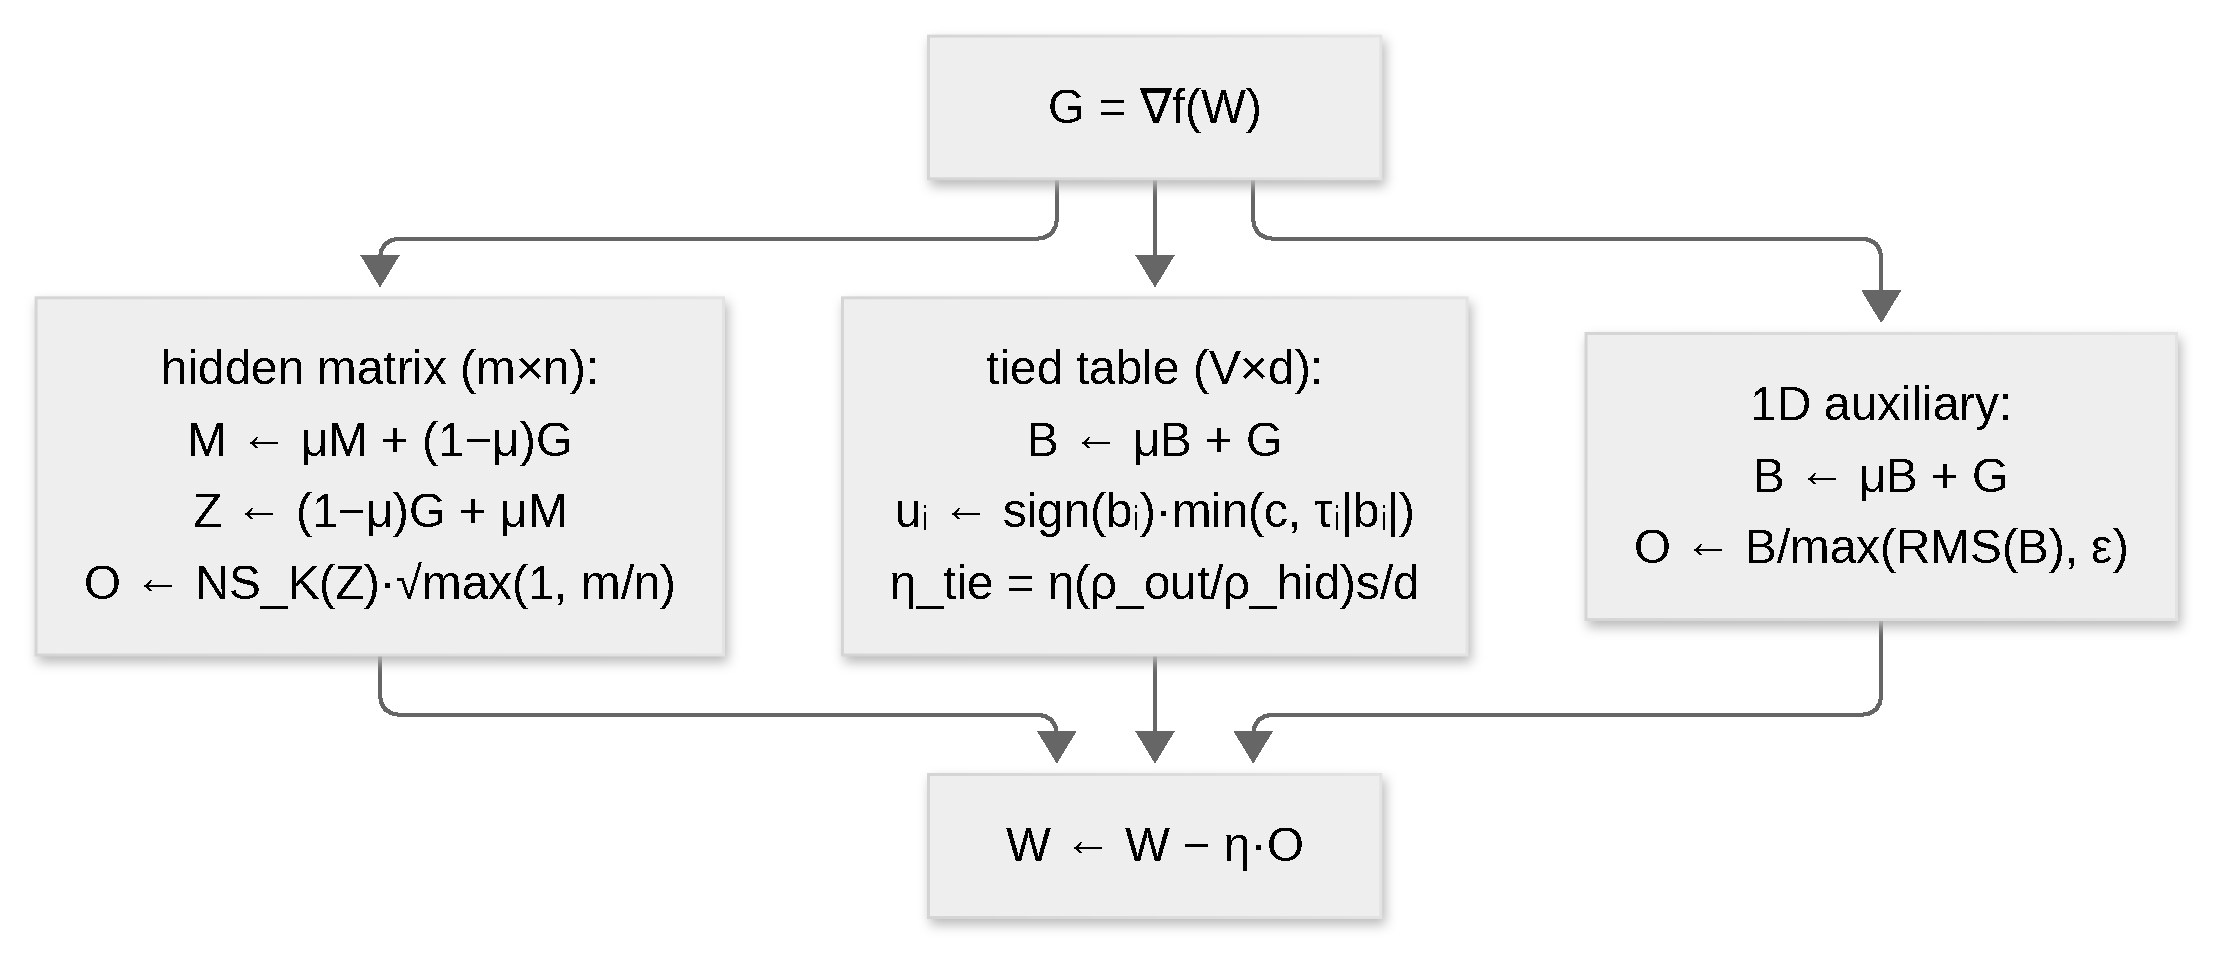
\includegraphics{../paper/figures/optimizers/af-muon.pdf}}
\caption{Flujo por paso de AF-Muon: actualización espectral de Muon para matrices ocultas, LMO por fila con tope finito y conciencia de soporte para la tabla de vocabulario atada, y actualizaciones normalizadas por RMS para parámetros auxiliares unidimensionales, todo con un único búfer de primer momento.}
\label{fig:opt-af-muon}
\end{figure}
AF-Muon es una \textbf{extensión de Muon sin AdamW} que elimina el respaldo auxiliar de AdamW de la receta Hybrid Muon asignando a cada clase de parámetro su propia geometría con restricción de norma. Las matrices ocultas conservan la actualización espectral con señal de Nesterov; la tabla de vocabulario, que recibe simultáneamente gradientes dispersos de búsqueda en la entrada y gradientes densos del softmax de salida, se actualiza fila por fila con un \emph{oráculo de minimización lineal con tope finito y conciencia de soporte}; los tensores auxiliares unidimensionales reciben una actualización normalizada por RMS. Ninguna clase de parámetro mantiene estado de segundo momento, de modo que un único búfer de primer momento por parámetro reemplaza el estado de AdamW de la receta híbrida, lo que los autores reportan como aproximadamente un 20\% menos de memoria de estado del optimizador en entrenamiento equiparado.

Para la tabla atada $W \in \mathbb{R}^{V \times d}$ con fila de momento $b_i$, el oráculo resuelve el problema por fila
\begin{align}
u_i &= \operatorname{sign}(b_i) \odot \min\left(c\,\mathbf{1},\ \tau_i\,|b_i|\right), \\
\|u_i\|_2^2 &= \min\left(d,\ c^2\,\bigl|\operatorname{supp}(b_i)\bigr|\right),
\end{align}
donde la escala por fila $\tau_i$ se obtiene por bisección en FP32 sobre fragmentos de filas completas. Las filas cuyo soporte no puede llenar el radio $\ell_2$ de fila saturan cada coordenada útil en el tope $c$, de modo que las filas dispersas de búsqueda se manejan sin inflar las coordenadas ausentes. El tope interpola entre dos extremos conocidos: $c = 1$ recupera la actualización Sign estilo SCION y $c \geq \sqrt{d}$ se reduce a una actualización row-RMS. El tamaño de paso de la tabla es $\eta_{tie} = \eta_M (\rho_{out}/\rho_{hid})\, s / d$; la configuración principal del artículo es $c = 3$ y $s = 0.5$ con $\rho_{out}/\rho_{hid} = 60$, y sus diagnósticos reportan el tope finito activo en menos del 0.3\% de las coordenadas aunque afecta a la mayoría de las filas.

\begin{algorithm}[H]
\caption{AF-Muon (Muon sin AdamW para Vocabulario Atado)}
\label{alg:af-muon}
\begin{algorithmic}[1]
\Require Parámetros iniciales $\theta$, LR de matrices $\eta_M$, LR de vectores $\eta_{vec}$, momento $\mu$, weight decay de matrices $\lambda_M$, escala de tabla $s$, tope $c$, radios $\rho_{out}, \rho_{hid}$, iteraciones Newton-Schulz $K$
\Ensure Parámetros actualizados $\theta_T$
\For{cada tensor de parámetros $W$ con gradiente $G_t$}
    \If{$W$ es una matriz oculta en $\mathbb{R}^{m \times n}$}
        \State $M_t \gets \mu M_{t-1} + (1-\mu) G_t$ \Comment{Primer momento}
        \State $Z_t \gets (1-\mu) G_t + \mu M_t$ \Comment{Señal de Nesterov}
        \State $O_t \gets \mathrm{NS}_K(Z_t)\sqrt{\max(1, m/n)}$ \Comment{Actualización espectral}
        \State $W_t \gets (1 - \eta_M \lambda_M) W_{t-1} - \eta_M O_t$
    \ElsIf{$W \in \mathbb{R}^{V \times d}$ es la tabla de vocabulario atada}
        \State $B_t \gets \mu B_{t-1} + G_t$ \Comment{Primer momento sin normalizar}
        \State $\eta_{tie,t} \gets \eta_M (\rho_{out}/\rho_{hid}) s / d$
        \For{cada fila $i = 1, \ldots, V$}
            \State $u_i \gets L_c\bigl(\mathrm{fila}_i(B_t)\bigr)$ \Comment{LMO por fila con tope}
        \EndFor
        \State $W_t \gets W_{t-1} - \eta_{tie,t} U$
    \Else
        \State $B_t \gets \mu B_{t-1} + G_t$ \Comment{Tensor auxiliar 1D}
        \State $O_t \gets B_t / \max(\mathrm{RMS}(B_t), \epsilon)$
        \State $W_t \gets W_{t-1} - \eta_{vec} O_t$
    \EndIf
\EndFor
\Return $\theta_T$
\end{algorithmic}
\end{algorithm}

\paragraph{Contras.}
\begin{itemize}[leftmargin=*]
\item Cada parámetro debe recibir un rol explícito (matriz, tabla atada o vector); un head de salida no atado o una tabla de embeddings adicional no son bloques de tabla atada.
\item El oráculo de la tabla requiere bisección por fila con fragmentación de filas completas; el artículo reporta aproximadamente un 1\% de sobrecarga mediana por paso en entrenamiento equiparado.
\item La afirmación sobre la tabla atada se establece para modelos con vocabulario atado; no se reclama preentrenamiento a escala frontera ni superioridad universal de los extremos.
\end{itemize}

\paragraph{Ventajas.}
\begin{itemize}[leftmargin=*]
\item Sin AdamW: un búfer de primer momento por parámetro y sin estado de segundo momento, reportado como aproximadamente un 20\% menos de memoria de estado del optimizador que Hybrid Muon.
\item El tope finito preserva las magnitudes intra-fila mientras acota la concentración de coordenadas, y recupera Sign ($c=1$) y row-RMS ($c \geq \sqrt{d}$) como casos límite.
\item Mejora la pérdida de validación y la perplejidad medias frente a Hybrid Muon y a un extremo Sign estilo SCION en nueve configuraciones de vocabulario atado que abarcan texto, tokens de imagen, proteínas, MoE y modelos encoder-decoder.
\end{itemize}

\paragraph{AdaMuon (Muon Adaptativo).}
AdaMuon es una \textbf{extensión adaptativa de Muon} que conserva la actualización espectral (polar) y añade normalización de varianza por coordenada. Muon ortogonaliza la matriz de momentum en una actualización puramente direccional, lo que elimina el escalado anisotrópico pero asigna la misma magnitud a todas las coordenadas; AdaMuon aborda el desajuste resultante entre coordenadas ruidosas e informativas siguiendo la varianza por elemento de la dirección \emph{ortogonalizada}, en lugar de la del gradiente crudo o la del momentum. Como el factor polar es globalmente invariante a escala, la transformación de signo aplicada antes de la ortogonalización preserva la dirección de la actualización mientras estabiliza sus magnitudes por elemento; el artículo demuestra que $\operatorname{sign}$ es la única aplicación elemental que es libre de escala, consistente con el signo, impar y acotada (Teorema~1). La estimación de segundo momento ve así una señal estable, y su versión normalizada por varianza se reescala a un RMS de $0.2$, igualando la escala empírica de actualización de Adam para reutilizar sin ajuste los schedules de tasa de aprendizaje existentes.

Para un peso $W_t \in \mathbb{R}^{n \times m}$, búfer de momentum $M_t$, momentum $\beta$, pasos de Newton--Schulz $T$ y constante pequeña $\varepsilon$:
\begin{align}
M_t &= \beta M_{t-1} + G_t, \\
O_t &= \operatorname{NewtonSchulz}\bigl(\operatorname{sign}(M_t), T\bigr), \\
V_t &= \beta V_{t-1} + (1-\beta)\, O_t \odot O_t, \\
\widehat{O}_t &= O_t \oslash \bigl(\sqrt{V_t} + \varepsilon \mathbf{1}\bigr), \\
\gamma_t &= \frac{0.2\sqrt{mn}}{\|\widehat{O}_t\|_F}, \\
W_{t+1} &= W_t - \eta\bigl(\gamma_t \widehat{O}_t + \lambda W_t\bigr).
\end{align}
El mapa de Newton--Schulz usa $X_0 = \operatorname{sign}(M_t)/\|\operatorname{sign}(M_t)\|_F$ y la iteración cúbica $X_k = aX_{k-1} + b(X_{k-1}X_{k-1}^{\mathsf T})X_{k-1} + c(X_{k-1}X_{k-1}^{\mathsf T})^2X_{k-1}$ con $(a,b,c) = (3.4445, -4.7750, 2.0315)$ y $T = 5$. No se aplica corrección de sesgo a ninguno de los momentos: un factor constante en $V_t$ se cancela exactamente con $\gamma_t \propto \sqrt{c}$, y un factor constante en $M_t$ se elimina con el mapa polar, $\operatorname{polar}(cM) = \operatorname{polar}(M)$.

\begin{algorithm}[H]
\caption{AdaMuon (Muon Adaptativo)}
\label{alg:ada-muon}
\begin{algorithmic}[1]
\Require Pesos iniciales $W_0 \in \mathbb{R}^{n \times m}$, tasa de aprendizaje $\eta$, weight decay $\lambda$, momentum $\beta$, pasos de Newton--Schulz $T$, constante pequeña $\varepsilon$
\Ensure Pesos actualizados $W_T$
\State $M_0 \gets \mathbf{0}$, $V_0 \gets \mathbf{0}$
\For{cada iteración $t = 1, 2, \ldots$}
    \State $G_t \gets \nabla_{W_t}\mathcal{L}(W_t)$
    \State $M_t \gets \beta M_{t-1} + G_t$
    \State $O_t \gets \operatorname{NewtonSchulz}(\operatorname{sign}(M_t), T)$
    \State $V_t \gets \beta V_{t-1} + (1-\beta)\, O_t \odot O_t$
    \State $\widehat{O}_t \gets O_t \oslash (\sqrt{V_t} + \varepsilon\mathbf{1})$
    \State $\gamma_t \gets 0.2\sqrt{mn}/\|\widehat{O}_t\|_F$
    \State $W_{t+1} \gets W_t - \eta(\gamma_t \widehat{O}_t + \lambda W_t)$
\EndFor
\Return $W_T$
\end{algorithmic}
\end{algorithm}

\paragraph{Contras.}
\begin{itemize}[leftmargin=*]
\item Un búfer de segundo momento adicional por parámetro matricial (dos búferes frente al único búfer de primer momento de Muon), más trabajo por paso de EMA elemental, raíz cuadrada y normalización sobre la actualización.
\item La actualización está definida para parámetros bidimensionales; los parámetros unidimensionales (sesgos, escalas de normalización) requieren un optimizador auxiliar en la receta del artículo.
\item El objetivo RMS ($0.2$) es una constante fija y no una cantidad aprendida, por lo que el método asume escalas de actualización tipo Adam al reutilizar schedules existentes.
\end{itemize}

\paragraph{Ventajas.}
\begin{itemize}[leftmargin=*]
\item Sin hiperparámetros nuevos: la EMA de segundo momento reutiliza el coeficiente de momentum $\beta$ de Muon, y el artículo reporta baja sensibilidad para $\beta \in [0.8, 0.99]$.
\item La transformación de signo hace que la estimación de varianza sea lo bastante estable para normalizar, y la alineación RMS cancela cualquier sesgo constante en $V_t$, por lo que no se necesita corrección de sesgo para ninguno de los dos momentos.
\item La alineación RMS iguala la escala de actualización de Adam, lo que permite reutilizar directamente los schedules de tasa de aprendizaje; los autores reportan hasta aproximadamente un 40\% de ganancia en eficiencia de entrenamiento frente a AdamW y mejoras consistentes frente a Muon en GPT-2 (125M--1.5B) y Qwen2.5 (1.5B, 7B).
\end{itemize}

\paragraph{Dion3 (Ortogonalización Fraccional con Gram-Newton-Schulz).}
Dion3~\citep{amsel_dion3_2026} es una \textbf{revisión de Muon} que reduce el costo del paso de ortogonalización a nivel algorítmico. Reemplaza Newton--Schulz estándar por \emph{Gram Newton--Schulz}, una iteración matemáticamente equivalente que opera sobre la pequeña matriz de Gram simétrica $XX^{\mathsf T}$, y ortogonaliza solo una fracción $f \in (0,1]$ de las filas del momentum en cada paso, actualizando únicamente esas filas de la matriz de pesos. El \emph{error feedback} decae solo las filas seleccionadas del búfer de momentum, de modo que las filas no seleccionadas siguen acumulándose y terminan siendo elegidas. Con $f = 1$ la actualización se reduce a Muon en aritmética exacta (o a NorMuon con la normalización por filas opcional). Para un peso $W \in \mathbb{R}^{n \times m}$ (operando sobre la dimensión menor, $n \le m$), fracción $f$, $k = \lceil f n \rceil$, momentum $\mu$, tasa de aprendizaje $\eta$ y weight decay $\lambda$:
\begin{align}
M_t &= M_{t-1} + G_t \quad\text{(acumulación de momentum; amortiguamiento diferido)} \\
S_t &= \operatorname{topk}_{i}\bigl(\lVert M_{t,i,:}\rVert_1,\ k\bigr) \quad\text{(seleccionar las } k \text{ filas mayores)} \\
O_t &= \operatorname{GramNS}\bigl(M_t[S_t,:]\bigr) \quad\text{(ortogonalizar la submatriz } k \times m\text{)} \\
W_t &= (1 - \eta\lambda)\, W_{t-1}, \qquad W_t[S_t,:] \gets W_t[S_t,:] - \eta\, O_t \\
M_t[S_t,:] &\gets \mu\, M_t[S_t,:] \quad\text{(error feedback: decaer solo las filas seleccionadas)}
\end{align}
Gram Newton--Schulz normaliza $X \gets M_t[S_t,:]/(\lVert M_t[S_t,:]\rVert_F + \epsilon)$ con $\epsilon = 10^{-7}$, convierte a \texttt{float16}, forma $R_0 = X X^{\mathsf T}$ y $Q_0 = I$, y ejecuta $T$ iteraciones
\begin{align}
Z_t &= b_t R_{t-1} + c_t R_{t-1}^2, &
Q_t &= Q_{t-1} Z_t + a_t Q_{t-1}, \\
(RZ)_t &= R_{t-1} Z_t + a_t R_{t-1}, &
R_t &= Z_t (RZ)_t + a_t (RZ)_t,
\end{align}
y devuelve $Q_T X$. Un \emph{reinicio} tras la iteración~2 ($X \gets Q_2 X$, $R_2 \gets X X^{\mathsf T}$, $Q_2 \gets I$) elimina los autovalores negativos espurios que la media precisión introduce en la matriz de Gram; los coeficientes $(a_t,b_t,c_t)$ son las ternas de cinco pasos de Polar Express~\citep{amsel_polar_express_2026}. El costo baja de $T(3\alpha+1)n^3$ FLOPs para Newton--Schulz estándar a $(4T+3\alpha-3)n^3$ para Gram Newton--Schulz ($\alpha = m/n$), y seleccionar $k = \lceil f n \rceil$ filas reduce la iteración y eleva la relación de aspecto en $1/f$. La variante NorMuon opcional añade un segundo momento por fila $v_i \gets \beta_2 v_i + (1-\beta_2)\,\operatorname{mean}_j(O_{ij}^2)$ para $i \in S$, reescala $\tilde O_{ij} = O_{ij}/(\sqrt{v_i}+\epsilon)$ y renormaliza $\tilde O \gets \tilde O\,\lVert O\rVert_F/\lVert\tilde O\rVert_F$ en \texttt{float32} antes de la actualización.

\begin{algorithm}[H]
\caption{Dion3 (Ortogonalización Fraccional con Retroalimentación de Error)}
\label{alg:dion3}
\begin{algorithmic}[1]
\Require Matrices $W$, tasa de aprendizaje $\eta$, momentum $\mu$, fracción $f$, pasos de Gram Newton--Schulz $T$, $\epsilon$, weight decay $\lambda$
\Ensure Matrices actualizadas $W_T$
\For{cada matriz de parámetros 2D $W$ con gradiente $G$}
    \State $M \gets M + G$ \Comment{Acumulación de momentum}
    \State $S \gets$ índices de las $k = \lceil f n \rceil$ filas de $M$ con mayor norma $\ell_1$ \Comment{Selección}
    \State $O \gets \operatorname{GramNS}_T(M[S,:])$ \Comment{Ortogonalizar la submatriz seleccionada}
    \If{NorMuon}
        \State $v_i \gets \beta_2 v_i + (1-\beta_2)\operatorname{mean}_j(O_{ij}^2)$ para $i \in S$
        \State $\tilde O_{ij} \gets O_{ij}/(\sqrt{v_i}+\epsilon)$; \quad $\tilde O \gets \tilde O\,\lVert O\rVert_F/\lVert\tilde O\rVert_F$
    \EndIf
    \State $W \gets (1 - \eta\lambda) W$ \Comment{Weight decay en todas las filas}
    \State $W[S,:] \gets W[S,:] - \eta\,\tilde O$ \Comment{Actualizar solo las filas seleccionadas}
    \State $M[S,:] \gets \mu\, M[S,:]$ \Comment{Error feedback}
\EndFor
\Return $W_T$
\end{algorithmic}
\end{algorithm}

\paragraph{Contras.}
\begin{itemize}[leftmargin=*]
\item Cada paso actualiza solo una fracción de las filas, por lo que la trayectoria de optimización difiere de Muon; el artículo reporta que el cambio es benigno (Sección~8.1 del reporte Dion3).
\item La selección de filas y el error feedback añaden contabilidad top-$k$ y un decaimiento del momentum por filas en cada paso.
\item Las mayores ganancias de tiempo de reloj del artículo provienen de kernels GEMM simétricos y comunicación megaagrupada, específicos de hardware y clúster; aquí solo aplican la reducción algorítmica y el único búfer de primer momento.
\end{itemize}

\paragraph{Ventajas.}
\begin{itemize}[leftmargin=*]
\item Gram Newton--Schulz es matemáticamente equivalente a Newton--Schulz y reduce los FLOPs de ortogonalización en torno al 55\% en relaciones de aspecto típicas de transformer con cinco iteraciones.
\item La selección fraccional de filas reduce la submatriz ortogonalizada a $k \times m$ y eleva su relación de aspecto en $1/f$, potenciando el ahorro de Gram; el artículo reporta pasos de optimizador hasta $6\times$ más rápidos con la misma pérdida.
\item Con $f = 1$ la actualización se reduce a Muon (o NorMuon), y basta un único búfer de momentum por parámetro matricial; el error feedback permite que las filas ignoradas participen eventualmente.
\end{itemize}

\paragraph{ROOT (Optimizador Ortogonalizado Robusto).}
\begin{figure}[H]
\centering
\fitfigure{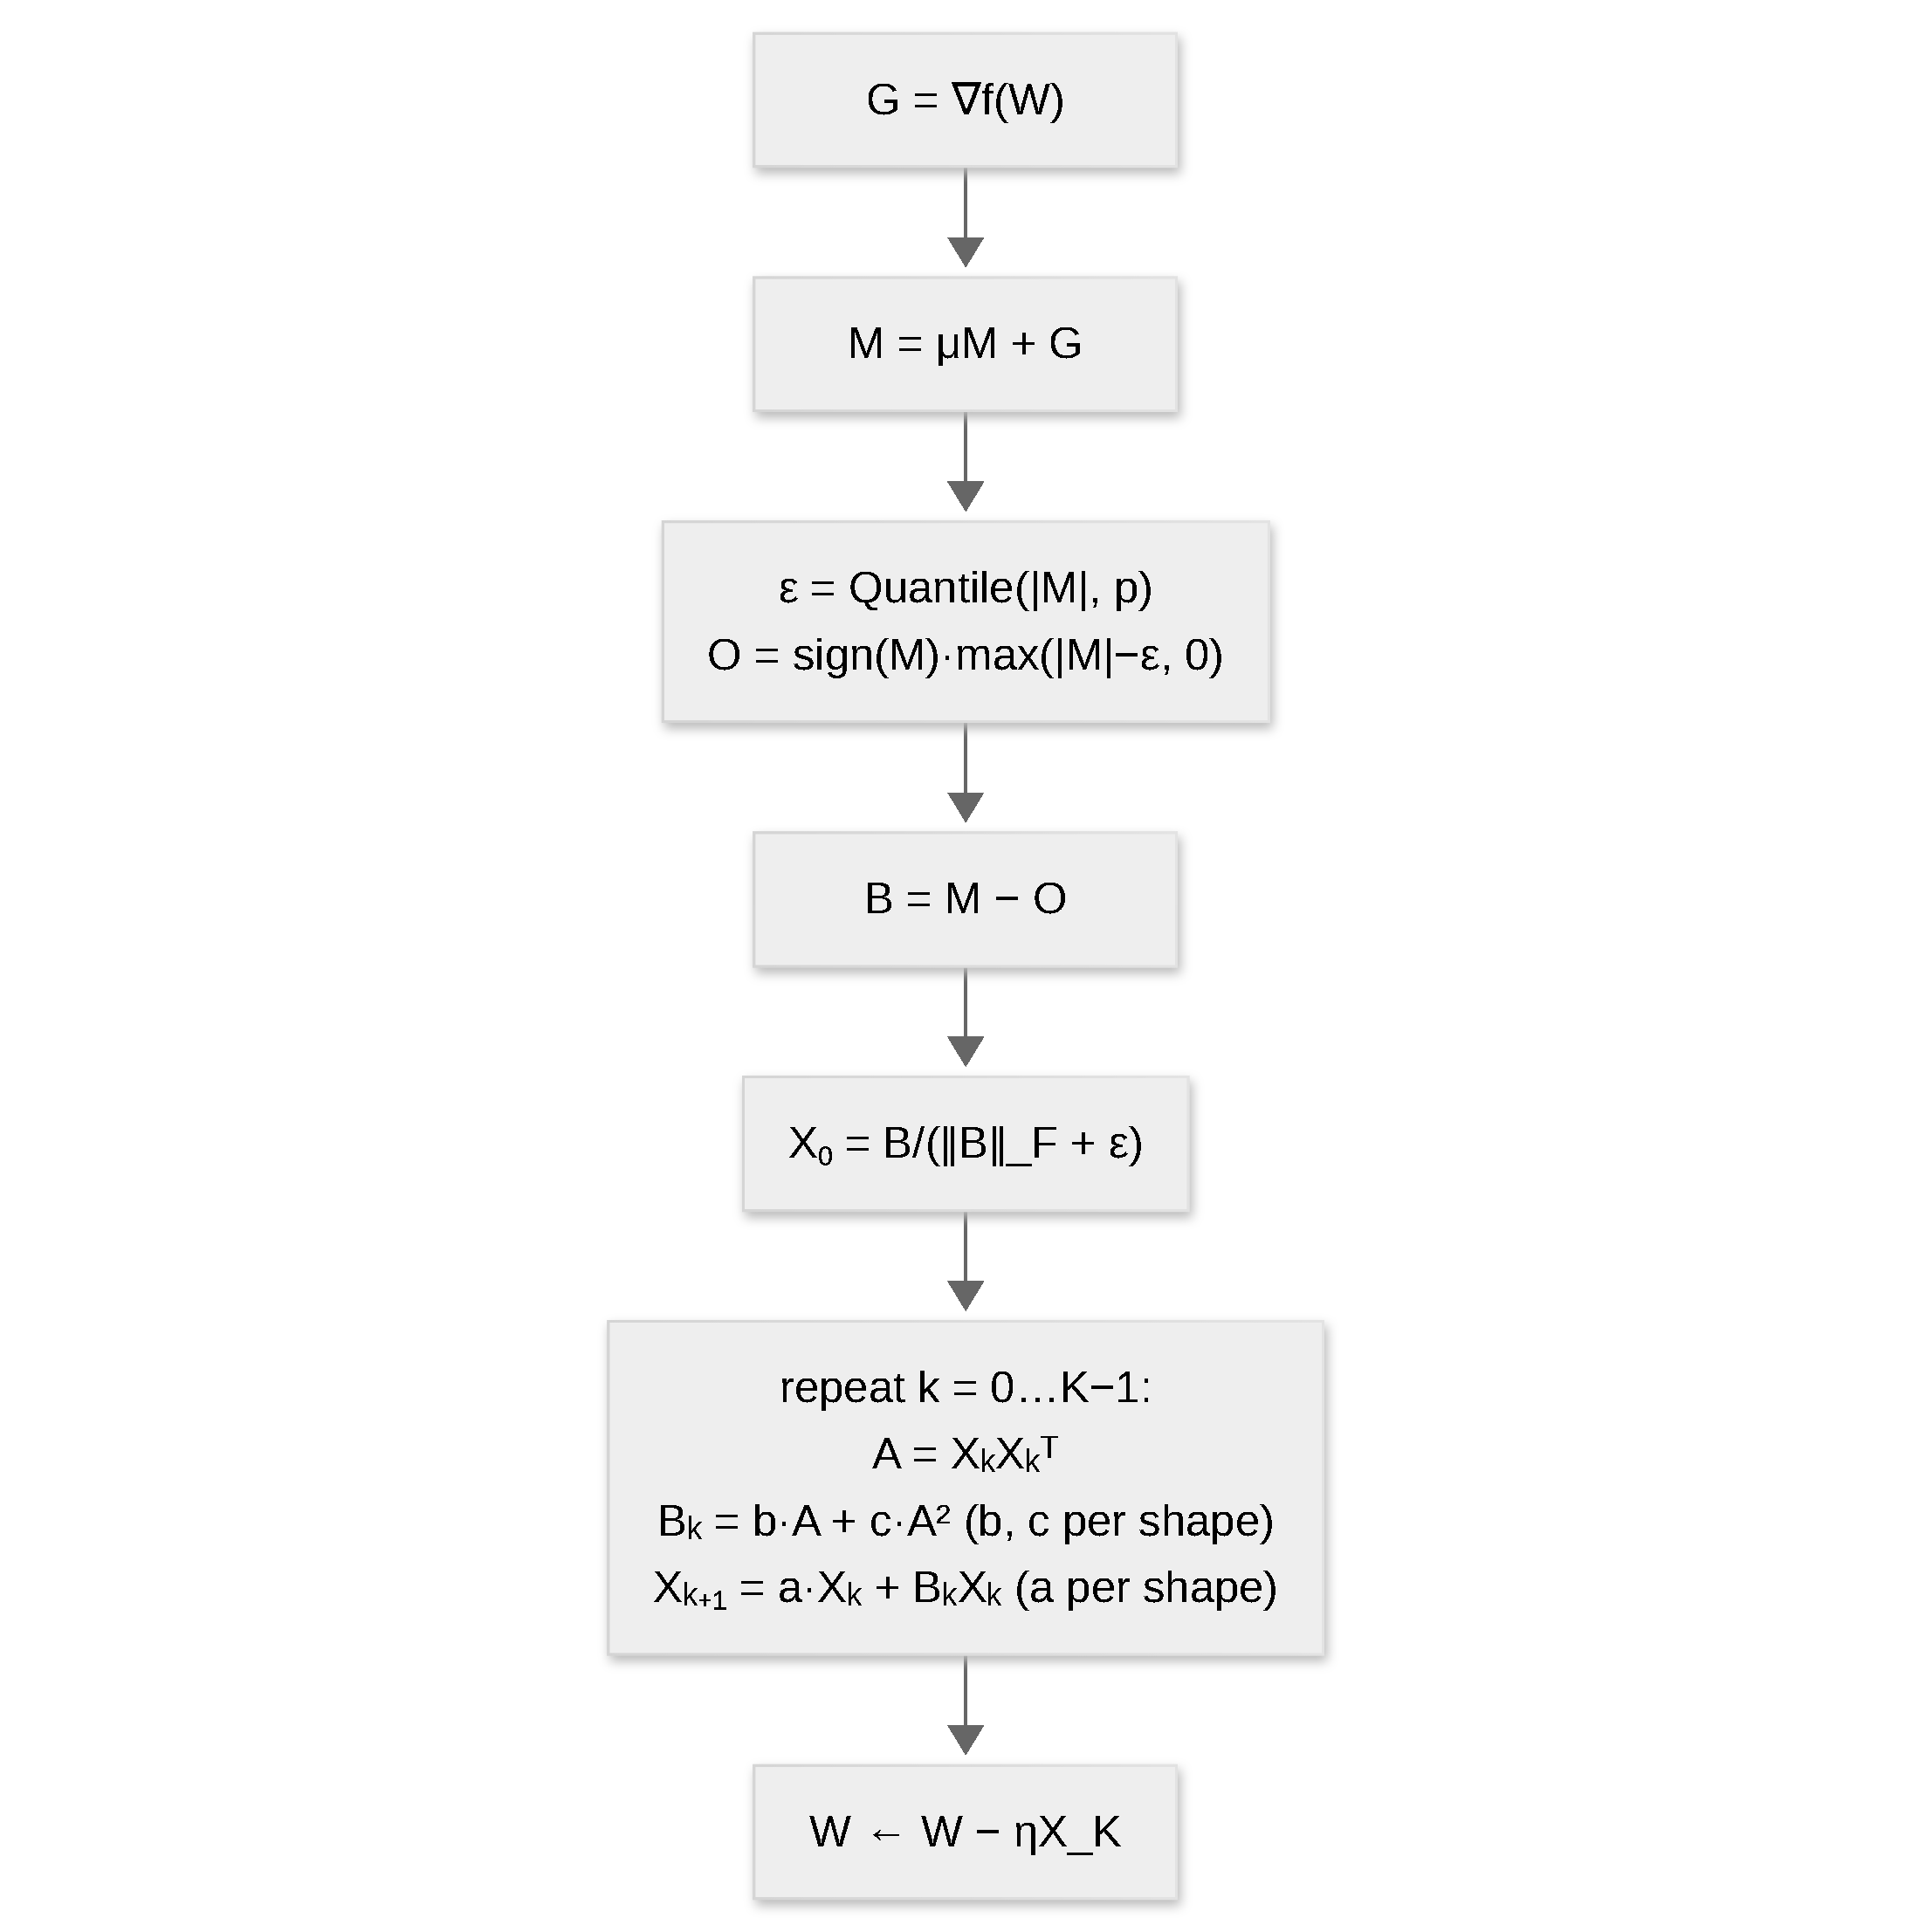
\includegraphics{../paper/figures/optimizers/root.pdf}}
\caption{Flujo por paso de ROOT: acumulación de momentum, separación de atípicos por soft-threshold y ortogonalización Newton--Schulz calibrada por forma.}
\label{fig:opt-root}
\end{figure}
ROOT~\citep{he_root_2025} es una \textbf{revisión orientada a la robustez de Muon} que ataca dos fragilidades del esquema Newton--Schulz de coeficientes fijos. Primero, los coeficientes universales $(a,b,c)=(3.4445,-4.7750,2.0315)$ están calibrados para una forma matricial ``promedio'' y pierden precisión justamente en capas cuadradas y casi cuadradas: el MSE de ortogonalización va de $0.0499$ en $2048\times2048$ a $0.0003$ en $2048\times16384$ en la Tabla~1 del artículo. ROOT los reemplaza por coeficientes por forma $\{a^{(m,n)}, b^{(m,n)}, c^{(m,n)}\}$ calibrados fuera de línea sobre distribuciones de valores singulares del momentum (calibración mixta 1:3 real-a-aleatorio), un esquema que los autores llaman \emph{AdaNewton}. Segundo, las componentes de gradiente de cola pesada distorsionan la normalización de Frobenius que requiere Newton--Schulz y son amplificadas por la iteración polinómica; ROOT modela el momentum como $M_t = B_t + O_t$ y resuelve un problema proximal L1 cuya solución cerrada es el soft-thresholding. Solo se ortogonaliza la componente base robusta $B_t$; la componente de atípicos dispersa $O_t$ se descarta. Para una matriz de pesos de capa oculta $W \in \mathbb{R}^{m\times n}$, momentum $\mu$, tasa de aprendizaje $\eta$, percentil $p$ e iteraciones $K$:
\begin{align}
M_t &= \mu M_{t-1} + \nabla \mathcal{L}(\theta_{t-1}) \quad\text{(momentum, Ec. 1)} \\
\varepsilon_t &= \operatorname{Quantile}(|M_t|, p) \quad\text{(umbral dinámico, } p=0.90 \text{ por defecto)} \\
O_t &= \mathcal{T}_{\varepsilon_t}[M_t], \quad \mathcal{T}_\varepsilon[x]_i = \operatorname{sign}(x_i)\max(|x_i|-\varepsilon, 0) \quad\text{(soft-threshold, Ecs. 7--10)} \\
B_t &= M_t - O_t \quad\text{(componente robusta recortada, Ec. 9)} \\
X_0 &= \frac{B_t}{\lVert B_t\rVert_F}, \qquad X_k = a^{(m,n)}X_{k-1} + b^{(m,n)}X_{k-1}(X_{k-1}^\top X_{k-1}) + c^{(m,n)}X_{k-1}(X_{k-1}^\top X_{k-1})^2 \\
\theta_t &= \theta_{t-1} - \eta X_K \quad\text{(actualización, } K=5\text{)}
\end{align}

\begin{table}[H]
\centering
\caption{Coeficientes AdaNewton de la Tabla~1 de \citet{he_root_2025} (calibración mixta 1:3). Las formas fuera de la tabla usan los coeficientes fijos de Muon $(3.4445,-4.7750,2.0315)$.}
\label{tab:root-coefficients}
\small
\begin{tabular}{rrrrrr}
\toprule
$m$ & $n$ & $a^{(m,n)}$ & $b^{(m,n)}$ & $c^{(m,n)}$ & MSE \\
\midrule
2048 & 2048 & 3.3334 & $-4.2591$ & 1.7791 & 0.0352 \\
4096 & 4096 & 3.3732 & $-4.6134$ & 2.0576 & 0.0470 \\
8192 & 8192 & 3.3886 & $-4.9026$ & 2.3105 & 0.0587 \\
3072 & 2048 & 2.9091 & $-3.8108$ & 1.8600 & 0.0024 \\
4096 & 2048 & 2.7739 & $-3.4911$ & 1.6992 & 0.0010 \\
8192 & 2048 & 2.5925 & $-3.0010$ & 1.4138 & 0.0003 \\
16384 & 2048 & 2.7045 & $-3.2335$ & 1.5336 & 0.0003 \\
\bottomrule
\end{tabular}
\end{table}

\begin{algorithm}[H]
\caption{ROOT (Optimizador Ortogonalizado Robusto)}
\label{alg:root}
\begin{algorithmic}[1]
\Require Parámetros iniciales $\theta$, tasa de aprendizaje $\eta$, momentum $\mu$, percentil $p$, iteraciones Newton--Schulz $K$
\Ensure Parámetros actualizados $\theta_T$
\For{cada parámetro $P$}
    \If{$P$ es una matriz 2D de capa oculta $W$}
        \State $G \gets \nabla f(W)$ \Comment{Gradiente}
        \State $M \gets \mu M + G$ \Comment{Acumulación de momentum}
        \State $\varepsilon \gets \operatorname{Quantile}(|M|, p)$ \Comment{Umbral dinámico}
        \State $O \gets \operatorname{sign}(M)\max(|M|-\varepsilon, 0)$ \Comment{Separación de atípicos (soft-threshold)}
        \State $B \gets M - O$ \Comment{Componente robusta recortada}
        \State $X_0 \gets \frac{B}{\|B\|_F + \epsilon}$ \Comment{Normalización por norma de Frobenius}
        \For{$k = 0, 1, \ldots, K-1$}
            \State $A_k \gets X_k X_k^\top$ \Comment{Gramiana}
            \State $B_k \gets b^{(m,n)} A_k + c^{(m,n)} A_k^2$ \Comment{Coeficientes calibrados por forma}
            \State $X_{k+1} \gets a^{(m,n)} X_k + B_k X_k$ \Comment{Paso polinómico}
        \EndFor
        \State $W \gets W - \eta X_K$ \Comment{Actualización con dirección ortogonalizada}
    \Else
        \State $P \gets \operatorname{AdamW}(P, \nabla f(P); \eta, \beta_1, \beta_2, \epsilon, \lambda)$ \Comment{Respaldo híbrido: embeddings, pos, heads, no matriciales}
    \EndIf
\EndFor
\Return $\theta_T$
\end{algorithmic}
\end{algorithm}

Siguiendo la receta híbrida de Muon, solo las matrices 2-D de capas ocultas toman la ruta ROOT; las tablas de embeddings, los encodings posicionales aprendidos, los heads de salida y todo parámetro no matricial se entrenan con AdamW desacoplado usando la tasa de aprendizaje, el weight decay, $\beta_1, \beta_2$ y $\epsilon$ por grupo. Los experimentos LLM del artículo aplican un factor de escalado de RMS de actualización de $0.2$ siguiendo Moonlight; esta implementación deja que las tasas de aprendizaje por grupo absorban esa calibración, por lo que no se aplica ninguna constante de escala. Las formas ausentes de la Tabla~\ref{tab:root-coefficients} usan los coeficientes fijos de Muon, y el cuantil dinámico cuesta un ordenamiento adicional de $|M_t|$ por matriz y por paso.

\paragraph{Contras.}
\begin{itemize}[leftmargin=*]
\item El umbral por percentil requiere un ordenamiento $O(N\log N)$ de la matriz de momentum en cada paso, además de las multiplicaciones de Newton--Schulz.
\item La tabla de coeficientes calibrados cubre solo siete formas; cualquier otra forma usa los coeficientes fijos de Muon.
\item Los atípicos se descartan en lugar de encogerse, por lo que un gradiente extremadamente ruidoso también puede perder señal informativa; la ablación del artículo muestra que el compromiso lo gobierna el percentil (0.85 recorta demasiado, 0.99 demasiado poco).
\end{itemize}

\paragraph{Ventajas.}
\begin{itemize}[leftmargin=*]
\item Precisión de ortogonalización invariante a la dimensión: los coeficientes calibrados por forma eliminan el precipicio de precisión que los coeficientes fijos muestran en capas cuadradas y casi cuadradas.
\item Robustez frente a atípicos sin reajustar la receta de Muon; el artículo reporta menor pérdida y mejor promedio zero-shot que Muon y AdamW a escala 1B (60.12 vs 59.59 vs 59.05) y ganancias en ViT/CIFAR-10.
\item El mismo único búfer de momentum por parámetro matricial que Muon, y los interruptores \texttt{softthresh}/\texttt{ada\_newton} exponen directamente las ablaciones del artículo.
\end{itemize}

\paragraph{Muon² (Ortogonalización con Precondicionamiento de Segundo Momento).}
Muon$^2$~\citep{liu_muon2_2026} generaliza Muon al precondicionar el momentum con un
\textbf{EMA de segundo momento estilo Adam antes de la ortogonalización de
Newton--Schulz}. El artículo muestra que el cuello de botella práctico de la aproximación
polar de Muon es la matriz de momentum mal condicionada (los espectros al inicio del
entrenamiento abarcan $10^{-4}$--$1$ y cerca de la mitad de los valores singulares caen en
la ``zona muerta'' de NS); dividir por $\sqrt{V_t}$ estrecha el espectro, de modo que cada
paso de NS se alinea mejor con la actualización ortogonalizada verdadera (similitud coseno
$0.916$ con $K{=}3$ frente a $0.931$ de Muon con $K{=}5$, y $0.975$ con $K{=}5$). Para una
matriz de pesos de capa oculta $W \in \mathbb{R}^{n \times m}$ con tasa de aprendizaje
$\eta$:
\begin{align}
M_t &= \beta_1 M_{t-1} + (1-\beta_1) G_t && \text{(EMA de momentum, Ec.~2)} \\
V_t &= \beta_2 V_{t-1} + (1-\beta_2)\, (G_t \odot G_t) && \text{(EMA de segundo momento, Ec.~3)} \\
\widetilde{M}_t &= M_t \oslash \big(\sqrt{V_t} + \epsilon \mathbf{1}\big) && \text{(precondicionamiento, Ec.~4)} \\
X_0 &= \frac{\widetilde{M}_t}{\|\widetilde{M}_t\|_F + \epsilon}, \qquad
X_{k+1} = aX_k + b\, X_k X_k^\top X_k + c\, X_k (X_k X_k^\top)^2 X_k && \text{(NS, Ec.~5)} \\
W_{t+1} &= W_t - \eta \sqrt{m/n}\, X_K && \text{(actualización, Ec.~6)}
\end{align}
con los mismos coeficientes quínticos $(a,b,c)=(3.4445,-4.7750,2.0315)$ que Muon y el
factor de tasa de aprendizaje $\sqrt{m/n}$ propuesto por Bernstein (2025). La variante
eficiente en memoria \textbf{Muon$^2$-F} reemplaza $V_t$ por estadísticas de fila/columna
estilo Adafactor:
\begin{align}
r_t &= \beta_2 r_{t-1} + (1-\beta_2)\,\mathrm{sum}_{\mathrm{col}}(G_t \odot G_t), \qquad
c_t = \beta_2 c_{t-1} + (1-\beta_2)\,\mathrm{sum}_{\mathrm{row}}(G_t \odot G_t), \\
\widehat{V}_t &= \frac{r_t\, c_t^\top}{\mathrm{sum}(r_t)},
\end{align}
manteniendo la memoria dentro de $\sim$0.3\% de Muon a escala 7B (47.53 vs 47.29 GB) y
conservando la mayor parte del beneficio de Muon$^2$. En preentrenamiento de GPT, LLaMA y
Mezcla de Expertos hasta 13B parámetros, Muon$^2$ supera a Muon con igual número de
iteraciones NS y lo iguala con $K{=}3$ en lugar de $5$ (una reducción del 40\%), ahorrando
hasta un cuarto del tiempo de entrenamiento con la misma pérdida.

\begin{algorithm}[H]
\caption{Muon² (Ortogonalización con Precondicionamiento de Segundo Momento)}
\label{alg:muon2}
\begin{algorithmic}[1]
\Require Parámetros iniciales $\theta$, tasa de aprendizaje $\eta$, $\beta_1, \beta_2$, iteraciones NS $K$, precondicionador $\epsilon$
\Ensure Parámetros actualizados $\theta_T$
\For{cada parámetro $P$}
    \If{$P$ es una matriz 2D de capa oculta $W \in \mathbb{R}^{n\times m}$}
        \State $G \gets \nabla f(W)$ \Comment{Gradiente}
        \State $M \gets \beta_1 M + (1-\beta_1) G$ \Comment{EMA de momentum (Ec.~2)}
        \State $V \gets \beta_2 V + (1-\beta_2) (G \odot G)$ \Comment{EMA de segundo momento (Ec.~3); la variante factorizada solo guarda sumas por fila/columna}
        \State $\widetilde{M} \gets M \oslash (\sqrt{V} + \epsilon\mathbf{1})$ \Comment{Precondicionar (Ec.~4)}
        \State $X_0 \gets \widetilde{M} / (\|\widetilde{M}\|_F + \epsilon)$ \Comment{Normalización por norma de Frobenius}
        \For{$k = 0, 1, \ldots, K-1$}
            \State $A_k \gets X_k X_k^\top$ \Comment{Gramiana}
            \State $X_{k+1} \gets 3.4445\,X_k - 4.7750\,A_k X_k + 2.0315\,A_k^2 X_k$ \Comment{Paso NS quíntico}
        \EndFor
        \State $W \gets W - \eta \sqrt{m/n}\, X_K$ \Comment{Actualización escalada (Ec.~6)}
    \Else
        \State $P \gets \operatorname{AdamW}(P, \nabla f(P); \eta, \beta_1, \beta_2, \epsilon, \lambda)$ \Comment{Respaldo híbrido: embeddings, pos, heads, no matriciales}
    \EndIf
\EndFor
\Return $\theta_T$
\end{algorithmic}
\end{algorithm}

Siguiendo la receta híbrida de Muon, solo las matrices 2-D de capas ocultas toman la ruta
Muon$^2$; las tablas de embeddings, los encodings posicionales aprendidos, las cabezas de
salida y todo parámetro no matricial se entrenan con AdamW desacoplado usando la tasa de
aprendizaje, el weight decay, $\beta_1, \beta_2$ y $\epsilon$ del grupo --- los mismos
$\beta_1, \beta_2, \epsilon$ que parametrizan las Ecs.~2--4, de modo que un único conjunto
de hiperparámetros por grupo configura ambas rutas.

\paragraph{Contras.}
\begin{itemize}[leftmargin=*]
\item Un búfer de estado completo adicional respecto de Muon (dos EMAs de momentos por
matriz), que duplica la memoria del optimizador en la ruta ortogonalizada salvo que se
active la variante factorizada.
\item La escala de actualización $\sqrt{m/n}$ difiere de la ruta \texttt{muon} simple de
este repositorio, por lo que las tasas de aprendizaje no se transfieren uno a uno entre
las dos entradas del registro.
\item El artículo no fija valores por defecto para $\beta_1, \beta_2$; esta implementación
hereda los valores compartidos por grupo $(0.9, 0.95)$.
\end{itemize}

\paragraph{Ventajas.}
\begin{itemize}[leftmargin=*]
\item Mejor ortogonalización con igual número de iteraciones NS y la misma calidad con un
40\% menos de iteraciones (3 en lugar de 5), recortando cómputo y comunicación de NS.
\item Ganancias consistentes sobre Muon en preentrenamiento de GPT, LLaMA y Mezcla de
Expertos hasta 13B parámetros, con hasta un cuarto del tiempo de entrenamiento ahorrado
con la misma pérdida.
\item El interruptor \texttt{factored} expone Muon$^2$-F, que mantiene la memoria dentro de
$\sim$0.3\% de Muon conservando la mayor parte del beneficio.
\end{itemize}

\paragraph{NorMuon (Muon Normalizado por Neurona).}
NorMuon~\citep{li_normuon_2025} conserva la actualización ortogonalizada de Muon y añade
sobre ella una \textbf{tasa de aprendizaje adaptativa por neurona (por fila)}. La
iteración Newton--Schulz de Muon iguala los valores singulares de la actualización, pero
la norma $L_2$ de las filas-neurona individuales sigue siendo muy no uniforme: algunas
neuronas reciben actualizaciones desproporcionadamente grandes mientras otras apenas se
entrenan. NorMuon registra la magnitud cuadrática media de cada fila de la dirección
\emph{ortogonalizada} en una EMA de segundo momento, divide cada fila-neurona por su RMS
y reescala toda la actualización a la escala empírica de Adam para que los schedules de
tasa de aprendizaje existentes se transfieran sin cambios. Para una matriz de pesos de
capa oculta $W \in \mathbb{R}^{m \times n}$ con tasa de aprendizaje $\eta$:
\begin{align}
M_t &= \beta_1 M_{t-1} + (1-\beta_1) G_t && \text{(momentum, línea 5)} \\
O_t &= \mathrm{NS}_5(M_t) && \text{(ortogonalización, línea 6)} \\
v_t &= \beta_2 v_{t-1} + (1-\beta_2)\,\mathrm{mean}_{\mathrm{cols}}(O_t \odot O_t) && \text{(EMA por neurona, línea 7)} \\
V_t &= \mathrm{ExpandRows}(v_t), \qquad \widehat{O}_t = O_t \oslash \big(\sqrt{V_t} + \epsilon\big) && \text{(normalización por fila, líneas 8--9)} \\
\hat\eta &= \frac{0.2\,\eta\,\sqrt{mn}}{\lVert \widehat{O}_t \rVert_F}, \qquad
W_{t+1} = W_t - \eta\lambda W_t - \hat\eta\,\widehat{O}_t && \text{(actualización, líneas 10--11)}
\end{align}
con $v_t \in \mathbb{R}^m$ (un escalar por neurona) y los mismos coeficientes quínticos
de Newton--Schulz $(a,b,c)=(3.4445,-4.7750,2.0315)$ que Muon. El estadístico por neurona
cuesta $m$ escalares frente al primer momento $m \times n$, así que el estado del
optimizador es $m(n+1)$ --- dentro de un factor $1/n$ de Muon y aproximadamente la mitad
del $2mn$ de Adam. En preentrenamiento de 1.1B y 5.4B, NorMuon necesita 21.74\% y 13.91\%
menos pasos que AdamW para alcanzar la misma pérdida de validación; en Modded-NanoGPT
(124M/350M) alcanza la pérdida de Muon con 6\% y 15\% menos iteraciones, con un sobrecosto
de 2.9\% en el tiempo por paso respecto de AdamW y 21.19 GB de estado del optimizador
frente a 40.56 GB de AdamW a 5.4B.

\begin{algorithm}[H]
\caption{NorMuon (Muon Normalizado por Neurona)}
\label{alg:normuon}
\begin{algorithmic}[1]
\Require Parámetros iniciales $\theta$, tasa de aprendizaje $\eta$, $\beta_1, \beta_2$, iteraciones NS $K$, $\epsilon$ de normalización por fila, weight decay $\lambda$
\Ensure Parámetros actualizados $\theta_T$
\For{cada parámetro $P$}
    \If{$P$ es una matriz 2D de capa oculta $W \in \mathbb{R}^{m\times n}$}
        \State $G \gets \nabla f(W)$ \Comment{Gradiente}
        \State $M \gets \beta_1 M + (1-\beta_1) G$ \Comment{Momentum (línea 5)}
        \State $O \gets \mathrm{NS}_K(M)$ \Comment{Newton--Schulz (línea 6)}
        \State $v \gets \beta_2 v + (1-\beta_2)\,\mathrm{mean}_{\mathrm{cols}}(O \odot O)$ \Comment{Segundo momento por neurona (línea 7)}
        \State $\widehat{O} \gets O \oslash (\sqrt{\mathrm{ExpandRows}(v)} + \epsilon\mathbf{1})$ \Comment{Normalización por fila (líneas 8--9)}
        \State $\hat\eta \gets 0.2\,\eta\,\sqrt{mn} / (\|\widehat{O}\|_F + \epsilon)$ \Comment{Alineación de RMS (línea 10)}
        \State $W \gets (1-\eta\lambda)\,W - \hat\eta\,\widehat{O}$ \Comment{Actualización (línea 11)}
    \Else
        \State $P \gets \operatorname{AdamW}(P, \nabla f(P); \eta, \beta_1, \beta_2, \epsilon, \lambda)$ \Comment{Respaldo híbrido: embeddings, pos, heads, no matriciales}
    \EndIf
\EndFor
\Return $\theta_T$
\end{algorithmic}
\end{algorithm}

Siguiendo la receta híbrida de Muon, solo las matrices 2-D de capas ocultas toman la ruta
NorMuon; las tablas de embeddings, los encodings posicionales aprendidos, los heads de
salida y todo parámetro no matricial se entrenan con AdamW desacoplado usando la tasa de
aprendizaje, el weight decay, $\beta_1, \beta_2$ y $\epsilon$ por grupo. Esta
implementación mapea los parámetros del artículo al registro así: el sufijo
\texttt{momentum} es $\beta_1$, el \texttt{betas[1]} compartido por grupo es $\beta_2$,
el \texttt{eps} compartido por grupo es $\epsilon$, y \texttt{ns\_steps}/\texttt{ns\_eps}
controlan la iteración Newton--Schulz. Como NS5 comienza con una normalización de
Frobenius, el escalado $(1-\beta_1)$ del momentum del artículo y la acumulación estándar
de momentum de este repositorio producen actualizaciones idénticas. El segundo aporte del
artículo, el Algoritmo~2, distribuye la ortogonalización entre rangos FSDP2 (asignación
round-robin de parámetros, gather/NS5/scatter y normalización por fila local al shard)
para evitar trabajo replicado; esa estrategia de despliegue es ortogonal a la regla de
actualización y no se implementa aquí.

\paragraph{Contras.}
\begin{itemize}[leftmargin=*]
\item Un vector de estado adicional por fila y por parámetro matricial (almacenado en
float32); pequeño frente al momentum $m \times n$, pero no nulo.
\item La normalización debe ir después de la ortogonalización: la ablación ``NorMuon
(Front)'' del artículo, que la aplica antes de NS5, es ligeramente peor.
\item $\epsilon$ se coloca fuera de la raíz ($\sqrt{V_t}+\epsilon$), siguiendo el
Algoritmo~2; la representación de la línea 9 en el Algoritmo~1 es tipográficamente
ambigua.
\item Los estadísticos por neurona no sustituyen el respaldo AdamW: embeddings, pos,
heads y tensores no 2-D siguen llevando primeros y segundos momentos completos.
\end{itemize}

\paragraph{Ventajas.}
\begin{itemize}[leftmargin=*]
\item Combina el bajo número de condición de Muon con normas de actualización por neurona
uniformes al estilo AdamW, superando consistentemente a ambos en preentrenamiento de
124M--5.4B.
\item El reescalado $0.2\eta\sqrt{mn}/\lVert\widehat{O}\rVert_F$ apunta a un RMS de
$0.2\eta$, por lo que los schedules de tasa de aprendizaje de Adam se aplican sin
reajuste.
\item La memoria se mantiene cerca de Muon ($m(n+1)$ frente a $mn$), aproximadamente la
mitad del estado del optimizador de Adam, y el sobrecosto por paso es de unos pocos por
ciento.
\end{itemize}

\paragraph{Conda (Adam Normalizado por Columnas).}
Conda~\citep{wang_conda_2025} conserva la adaptividad por coordenada de Adam y añade una
\textbf{normalización espectral más suave y específica por columna}. Los autores
reformulan primero Muon como un método de primer/segundo momento cuyo segundo momento es
la matriz constante por filas $\mathrm{diag}(\mathbf{\Sigma}_t)\mathbf{1}^\top$: Muon
normaliza cada columna de la actualización con los mismos factores $1/\sigma_i$, lo que
sobre-amplifica las direcciones con valores singulares diminutos. Conda restringe el
segundo momento al mismo subespacio que el primer momento proyectando el gradiente
estocástico, manteniendo una EMA por elemento de los \emph{gradientes proyectados al
cuadrado} y dividiendo el primer momento proyectado por su raíz cuadrada. Para una matriz
de pesos $W \in \mathbb{R}^{m \times n}$ con $m \le n$, tasa de aprendizaje $\eta$,
decaimientos $\beta_1,\beta_2$, periodo de refresco del subespacio $T$, factor de escala
$\alpha$ y constante de estabilidad $\epsilon$:
\begin{align}
M_t &= \beta_1 M_{t-1} + (1-\beta_1) G_t \\
\bar U_t &=
\begin{cases}
\mathrm{SVD}(M_t), & t \bmod T = 0, \\
\bar U_{t-1}, & \text{en otro caso},
\end{cases} \\
M'_t &= \bar U_t^\top M_t, \qquad
N_t = \beta_2 N_{t-1} + (1-\beta_2)\big(\bar U_t^\top G_t\big)^2, \\
\widehat M_t &= \frac{M'_t}{1-\beta_1^t}, \qquad
\widehat N_t = \frac{N_t}{1-\beta_2^t}, \\
W_t &= W_{t-1} - \eta\,\alpha\,\bar U_t\,
      \frac{\widehat M_t}{\sqrt{\widehat N_t} + \epsilon}.
\end{align}
Para $m > n$ la base singular derecha $V_t$ reemplaza a $\bar U_t$ ($M'_t = M_t V_t$,
$N_t$ rastrea $(G_t V_t)^2$ y la actualización es
$(\widehat M_t/\sqrt{\widehat N_t})\,V_t^\top$), exactamente como en la implementación de
referencia publicada. La SVD es el único paso superlineal y se ejecuta cada $T$ pasos
($T=2000$ en el preentrenamiento del artículo, $T=200$ en sus ejecuciones LoRA); el
sobrecosto en tiempo de reloj es despreciable para $T \ge 100$.

\begin{algorithm}[H]
\caption{Conda (Adam Normalizado por Columnas)}
\label{alg:conda}
\begin{algorithmic}[1]
\Require Parámetros $\theta$, tasa de aprendizaje $\eta$, $\beta_1,\beta_2$, periodo de refresco $T$, escala $\alpha$, $\epsilon$, weight decay $\lambda$
\Ensure Parámetros actualizados $\theta_T$
\For{cada parámetro $P$}
    \If{$P$ es una matriz 2-D $W \in \mathbb{R}^{m\times n}$}
        \State $G \gets \nabla f(W)$ \Comment{Gradiente}
        \State $M \gets \beta_1 M + (1-\beta_1) G$ \Comment{Primer momento}
        \If{$t \bmod T = 0$ o $P$ no tiene base}
            \State $U,\Sigma,V^\top \gets \mathrm{SVD}(M)$;\; $\bar U \gets U$ si $m\le n$, si no $V$ \Comment{Subespacio perezoso}
        \EndIf
        \State $G_{\mathrm{proj}} \gets \bar U^\top G$;\; $M_{\mathrm{proj}} \gets \bar U^\top M$ \Comment{Proyectar}
        \State $N \gets \beta_2 N + (1-\beta_2)\, G_{\mathrm{proj}}^2$ \Comment{Segundo momento proyectado}
        \State $M_{\mathrm{proj}} \gets M_{\mathrm{proj}}/(1-\beta_1^t)$;\; $N \gets N/(1-\beta_2^t)$ \Comment{Corrección de sesgo}
        \State $W \gets (1-\eta\lambda) W - \eta\,\alpha\,\bar U\, M_{\mathrm{proj}}/(\sqrt{N}+\epsilon)$ \Comment{Actualización}
    \Else
        \State $P \gets \operatorname{AdamW}(P, \nabla f(P); \eta, \beta_1, \beta_2, \epsilon, \lambda)$ \Comment{Respaldo no matricial}
    \EndIf
\EndFor
\Return $\theta_T$
\end{algorithmic}
\end{algorithm}

En preentrenamiento de LLaMA 60M--1B, Conda alcanza perplejidades de validación de 28.32,
21.38, 16.44 y 13.59, frente a 34.06/25.08/18.80/15.56 de AdamW y 29.89/22.15/16.51/14.17
de Muon, es decir, 2--2,5$\times$ la velocidad de convergencia de AdamW en pasos y en
tiempo de reloj; también lidera en GPT-2 (125M/355M: 17.40/13.92) y en el ajuste fino
LoRA de sentido común. A diferencia de AdamW y Muon, permanece estable con tasas de
aprendizaje de hasta $2\times10^{-2}$, y las ablaciones muestran robustez a
$T \in [2, 20000]$, $\beta_1 \in \{0.9, 0.95\}$ y
$\beta_2 \in \{0.95,\ldots,0.999\}$. La memoria del optimizador se mantiene a
0,03--1,3\,GB de AdamW de 60M a 1B. En esta implementación, el sufijo
\texttt{update\_proj\_gap} es $T$ (por defecto 2000), \texttt{scale} es $\alpha$ (por
defecto 1.0; el preentrenamiento del artículo usa 0.25), \texttt{correct\_bias} activa o
desactiva las correcciones $1-\beta^t$, y los \texttt{betas}/\texttt{eps} compartidos por
grupo son $(\beta_1,\beta_2)$ (el artículo usa 0.9/0.99) y $\epsilon$; el \texttt{wd}
compartido es desacoplado. Toda matriz 2-D toma la ruta Conda sin distinción de grupo ---
no hay exclusión de embeddings/pos/heads como en Muon --- mientras que todo parámetro no
2-D se entrena con AdamW desacoplado.

\paragraph{Contras.}
\begin{itemize}[leftmargin=*]
\item La SVD es un pico de costo por matriz cada $T$ pasos; con $T=2$ eleva el tiempo de
  reloj de LLaMA-60M de 2h49min a 4h37min.
\item El segundo momento debe vivir en el mismo subespacio que el primero: el estimador
  de Adam sin proyectar es inestable a escala y no converge en LLaMA-1B.
\item El estado del optimizador es del tamaño de Adam (primer momento $m\times n$
  completo) más la base de proyección; la ventaja de memoria frente a AdamW es pequeña,
  no el $O(nr)$ de GaLore.
\item Evaluado solo hasta 1B parámetros y sin Mezcla de Expertos; el artículo señala
  ambos como trabajo futuro.
\end{itemize}

\paragraph{Ventajas.}
\begin{itemize}[leftmargin=*]
\item Combina la adaptividad por coordenada de Adam con un mejor acondicionamiento
  espectral en una sola regla de actualización, superando consistentemente a AdamW,
  Muon, SOAP y Adafactor.
\item El normalizador por columna es más suave que el escalado uniforme $1/\sigma_i$ de
  Muon y preserva el orden relativo de los valores singulares, evitando sobrepasos en
  direcciones de valor singular pequeño.
\item Un único juego de hiperparámetros se transfiere de 60M a 1B, y el entrenamiento es
  estable con tasas de aprendizaje 10--20$\times$ mayores que las de AdamW.
\item La memoria y el costo por paso se mantienen cerca de AdamW para $T \gg 1$; la SVD
  perezosa hace que el refresco del subespacio sea casi gratuito en tiempo de reloj.
\end{itemize}

\paragraph{TUON (Optimización Consciente de Tensores vía T-SVD y Polarización).}
TUON~\citep{tang_tuon_2026} eleva la ortogonalización por capa de Muon a
\textbf{tensores entre capas} mediante un álgebra tensorial basada en transformaciones,
derivada del Tensor-SVD. Los mapas polares por capa descartan las correlaciones entre
capas, mientras que los optimizadores tensoriales basados en despliegue (TEON) sufren
desequilibrio de dimensiones y desalineación entre capas, y degradan más allá de dos
capas apiladas o de los módulos QKV. TUON en cambio \emph{mezcla y luego separa}: para
un grupo compatible de $K$ matrices de la misma forma con momentum apilado
$\mathcal{M}_t \in \mathbb{R}^{m \times n \times K}$:
\begin{align}
\mathcal{M}_t &= \beta \mathcal{M}_{t-1} + (1-\beta)\, \mathcal{G}_t
  && \text{(tensor de momentum, Alg.~1 línea 2)} \\
C_t &= \mathsf{M}_t \mathsf{M}_t^{\top} \in \mathbb{R}^{K \times K}, \qquad
C_t = U_t \Lambda_t U_t^{\top}, \qquad Q_t = U_t^{\top}
  && \text{(Gram de capas + autodescomposición, líneas 3--5)} \\
\widetilde{\mathcal{M}}_t &= \mathcal{M}_t \times_3 Q_t, \qquad
\widetilde{P}_{t,j} = \operatorname{polar}\!\big(\widetilde{\mathcal{M}}_{t,j}\big)
  && \text{(transformación + polarización por slice, líneas 6--9)} \\
\mathcal{P}_t &= \widetilde{\mathcal{P}}_t \times_3 Q_t^{H}
  && \text{(transformación inversa, línea 10)} \\
W_{t+1} &= (1 - \eta_t \lambda)\, W_t - \eta_t \gamma_t \mathcal{P}_t, \qquad
\gamma_t = \frac{s}{\operatorname{RMS}(\mathcal{P}_t) + \epsilon}
  && \text{(actualización escalada por RMS, línea 11)}
\end{align}
donde $\mathsf{M}_t$ es el despliegue por modo 3 (la $k$-ésima fila es
$\operatorname{vec}(\mathcal{M}_t^{(k)})^{\top}$), el producto por modo 3 mezcla los
slices como $\widetilde{\mathcal{M}}_{t,j} = \sum_k (Q_t)_{jk} \mathcal{M}_t^{(k)}$,
$\operatorname{RMS}(\mathcal{P}_t) = \sqrt{(mnK)^{-1} \sum_{i,j,k} |\mathcal{P}_t(i,j,k)|^2}$
y el RMS objetivo de la pila es $s = 1/\sqrt{\max(m,n)}$ (identidad rango--energía: slices
de rango completo dan $\operatorname{RMS} = 1/\sqrt{\max(m,n)}$, de modo que $\gamma_t
\approx 1$ y la magnitud de la actualización por matriz coincide con Muon). La
transformación por defecto \textbf{DecorQ} toma los autovectores de la matriz de Gram de
capas ($Q_t = U_t^{\top}$) y se refresca cada $T$ pasos (200 por defecto); diagonaliza la
Gram transformada, por lo que los slices transformados son mutuamente ortogonales en
Frobenius y cada mapa polar actúa en su propio subespacio: el problema acoplado de $K$
capas se desacopla en $K$ problemas de un solo canal. Las transformaciones unitarias
fijas (DCT, Haar, DFT) son válidas pero imponen un prior ajeno a la estadística de las
capas; en la ablación del artículo DecorQ (2.7598) supera a DFT (2.7631), Haar (2.7635),
DecorQ estático (2.7658) y DCT (2.8100) en Qwen3-4B. La polarización por slice usa la
misma iteración quíntica de Newton--Schulz que Muon, $(a,b,c) = (3.4445, -4.7750,
2.0315)$ con $J = 5$ pasos tras una normalización Frobenius y una transposición cuando la
matriz es alta.

\begin{algorithm}[H]
\caption{TUON (Optimización Consciente de Tensores vía T-SVD y Polarización)}
\label{alg:tuon}
\begin{algorithmic}[1]
\Require Matrices compatibles $\{W^{(k)}\}_{k=1}^{K}$, tasa de aprendizaje $\eta$, momentum $\beta$, weight decay $\lambda$, iteraciones NS $J$, intervalo de refresco $T$, $\epsilon$ del RMS
\Ensure Parámetros actualizados
\For{cada grupo compatible}
    \State $\mathcal{G} \gets \operatorname{stack}_3(\nabla f(W^{(1)}), \ldots, \nabla f(W^{(K)}))$ \Comment{Tensor de gradientes (línea 1)}
    \State $\mathcal{M} \gets \beta \mathcal{M} + (1-\beta)\, \mathcal{G}$ \Comment{Tensor de momentum (línea 2)}
    \State $C \gets \mathsf{M}\mathsf{M}^{\top}$; $C = U \Lambda U^{\top}$; $Q \gets U^{\top}$ \Comment{Gram + autodescomposición, refrescada cada $T$ pasos (líneas 3--5)}
    \State $\widetilde{\mathcal{M}} \gets \mathcal{M} \times_3 Q$ \Comment{Mezcla de slices (línea 6)}
    \For{$j = 1, \ldots, K$ en paralelo}
        \State $\widetilde{P}_{:, :, j} \gets \mathrm{NS}_J(\widetilde{\mathcal{M}}_{:, :, j})$ \Comment{Polarización por slice (líneas 7--9)}
    \EndFor
    \State $\mathcal{P} \gets \widetilde{\mathcal{P}} \times_3 Q^{H}$ \Comment{Transformación inversa (línea 10)}
    \State $\gamma \gets s / (\operatorname{RMS}(\mathcal{P}) + \epsilon)$ \Comment{Escala compartida de la pila (línea 11)}
    \State $W \gets (1-\eta\lambda) W - \eta \gamma \mathcal{P}$ \Comment{Actualización desacoplada (línea 11)}
\EndFor
\end{algorithmic}
\end{algorithm}

Esta implementación mapea el «grupo compatible» del artículo a cada cubeta
\emph{(grupo de parámetros, forma de matriz)}: las matrices 2-D ocultas de la misma forma
de un grupo se apilan por el modo de capas en orden de registro (\texttt{stack: full});
\texttt{stack: pairs} restringe la pila a pares consecutivos ($K=2$). El sufijo
\texttt{transform} selecciona $Q$ (\texttt{decorq} por defecto;
\texttt{dct}/\texttt{haar}/\texttt{dft} fijas), \texttt{momentum} es $\beta$,
\texttt{refresh\_interval} es $T$, \texttt{ns\_steps}/\texttt{ns\_eps} dirigen
Newton--Schulz y \texttt{rms\_eps} es el $\epsilon$ de $\gamma_t$. Con $K=1$ la
transformación se cancela exactamente y TUON se reduce a Muon (Prop.~2 del artículo);
siguiendo la receta híbrida de Muon, solo las matrices 2-D de capas ocultas toman la ruta
TUON: las tablas de embeddings, los encoding posicionales aprendidos, los heads de salida
y todo parámetro no matricial se entrenan con AdamW desacoplado usando el learning rate,
weight decay, $\beta_1, \beta_2$ y $\epsilon$ del grupo. Teoría: TUON es descenso máximo
bajo la norma espectral tensorial transformada por $Q$ (par dual
$\|\cdot\|_{Q,Ts}$ / $\|\cdot\|_{Q,Tn}$), su actualización es el factor polar tensorial
de una T-SVD de producto-T, ninguna transformación unitaria de capas distorsiona la
geometría de Muon en más de $\sqrt{K}$, y a radio de operador común el oráculo de TUON
nunca es más débil que el de TEON y puede ser hasta $\sqrt{K}$ más fuerte, con un
certificado de convergencia $O(T^{-1/2})$. Empíricamente TUON supera a Muon y TEON en
GPT-124M/350M y Qwen-0.6B/4B (pérdida de validación 2.9357/2.6925/2.8887/2.7598), es el
único método que mejora al pasar de $K{=}2$ a $K{=}\mathrm{full}$ en los cuatro modelos,
se transfiere de QKV a QKVO+MLP, y cuesta 0,2--1,1\% de tiempo de paso sobre TEON y a lo
sumo 12,5\% sobre AdamW; la complejidad por iteración es
$\mathcal{O}(Kmn\min(m,n) + K^2 mn)$, el mismo término dominante que Muon.

\paragraph{Contras.}
\begin{itemize}[leftmargin=*]
\item La mezcla entre capas asume matrices genuinamente compatibles; esta implementación
  apila por forma exacta dentro de un grupo de parámetros, la realización fiel más
  cercana disponible a partir de las listas de parámetros sin nombre de la factoría.
\item La Gram/autodescomposición añade $\mathcal{O}(K^2 mn)$ por paso y una base
  $K \times K$ por cubeta; despreciable para $K \ll \min(m, n)$, pero es un costo por
  cubeta que Muon no paga.
\item $\beta$ es requerido por el Algoritmo 1 pero su valor por defecto no aparece en el
  artículo; esta implementación hereda la convención de la familia Muon del repositorio
  ($0.95$).
\item La transformación \texttt{dft} ejecuta Newton--Schulz sobre slices complejos
  (Gram hermítica); se toma la parte real tras la transformación inversa, justificado por
  la simetría conjugada de la DFT de una pila real.
\end{itemize}

\paragraph{Ventajas.}
\begin{itemize}[leftmargin=*]
\item Explota la estructura entre capas que el Muon por capa descarta, con garantía de
  convergencia e interpretación exacta de descenso máximo bajo la norma tensorial
  inducida.
\item DecorQ depende de los datos y se refresca cada $T$ pasos; apilar
  $K{=}\mathrm{full}$ \emph{mejora} con la profundidad en lugar de degradar como ocurre
  con los métodos de despliegue.
\item La memoria se mantiene al nivel de Muon (un búfer de momentum por matriz más una
  base $K \times K$) y el escalado RMS de la pila conserva la magnitud de Muon, por lo que
  los learning rates existentes se transfieren.
\item Se aplica uniformemente más allá de QKV (atención, MLP y proyecciones de salida),
  donde los optimizadores tensoriales previos no se transfieren.
\end{itemize}

\paragraph{NAMO (Estimación Adaptativa de Momentos Basada en Normas con Momentum Ortogonalizado).}
NAMO~\citep{zhang_namo_2026} conserva la dirección de actualización ortogonalizada de
Muon y le añade una \textbf{adaptación al ruido tipo Adam basada en normas}. La
ortogonalización de matrices es una operación no acotada que puede amplificar el ruido
estocástico, por lo que el tamaño de paso efectivo de Muon no se reduce cuando los
gradientes se vuelven ruidosos. NAMO rastrea una EMA escalar del cuadrado de la norma de
Frobenius del gradiente y reescala toda la actualización ortogonalizada mediante el
cociente de normas con corrección de sesgo
$\lVert\widehat M_t\rVert_F/(\sqrt{\widehat v_t}+\epsilon_t)$ --- un estadístico de
señal-ruido agregado análogo al cociente por coordenada de Adam. Como el escalado es un
único escalar, la dirección de actualización permanece exactamente ortogonal, y el
estado del optimizador crece en un solo escalar por matriz respecto de Muon. Para una
matriz de pesos de capa oculta $W \in \mathbb{R}^{m\times n}$ con tasa de aprendizaje
$\eta$, momenta $\mu_1,\mu_2 \in [0,1)$, constante de estabilidad $\epsilon$ y weight
decay desacoplado $\lambda$:
\begin{align}
M_t &= \mu_1 M_{t-1} + (1-\mu_1) G_t && \text{(momentum)} \\
v_t &= \mu_2 v_{t-1} + (1-\mu_2)\,\lVert G_t\rVert_F^2 && \text{(EMA escalar de normas)} \\
O_t &= \mathrm{NS}_K(M_t) && \text{(ortogonalización)} \\
\alpha_t &= \frac{\sqrt{1-\mu_2^t}}{1-\mu_1^t}\cdot\frac{\lVert M_t\rVert_F}{\sqrt{v_t}+\epsilon}
   = \frac{\lVert\widehat M_t\rVert_F}{\sqrt{\widehat v_t}+\epsilon_t},
   \qquad \epsilon_t := \frac{\epsilon}{\sqrt{1-\mu_2^t}} && \text{(paso adaptativo)} \\
W_t &= W_{t-1} - \eta\,\alpha_t\,\bigl(O_t + \lambda W_{t-1}\bigr) && \text{(actualización)}
\end{align}
con los mismos coeficientes quínticos de Newton--Schulz $(a,b,c)=(3.4445,-4.7750,2.0315)$
que Muon. Bajo suavidad en norma nuclear y ruido de varianza acotada, NAMO alcanza la
tasa determinista óptima $\mathcal{O}(T^{-1/2})$, y su cota estocástica se descompone en
un término de optimización $\mathcal{O}(T^{-1/4})$ más un término de varianza
$\mathcal{O}(\sqrt{\sigma}\,b^{-1/4}T^{-1/8})$, recuperando la óptima $\mathcal{O}(T^{-1/4})$
cuando el tamaño de lote cumple $b=\Omega(\sigma^2 T^{1/2})$.

\begin{algorithm}[H]
\caption{NAMO (Estimación Adaptativa de Momentos Basada en Normas con Momentum Ortogonalizado)}
\label{alg:namo-es}
\begin{algorithmic}[1]
\Require Parámetros $\theta$, tasa de aprendizaje $\eta$, momenta $\mu_1,\mu_2$, iteraciones NS $K$, constante de estabilidad $\epsilon$, weight decay $\lambda$
\Ensure Parámetros actualizados $\theta_T$
\For{cada parámetro $P$}
    \If{$P$ es una matriz 2D de capa oculta $W \in \mathbb{R}^{m\times n}$}
        \State $G \gets \nabla f(W)$ \Comment{Gradiente}
        \State $M \gets \mu_1 M + (1-\mu_1) G$ \Comment{Momentum}
        \State $v \gets \mu_2 v + (1-\mu_2)\,\lVert G\rVert_F^2$ \Comment{Segundo momento escalar}
        \State $O \gets \mathrm{NS}_K(M)$ \Comment{Newton--Schulz}
        \State $\alpha \gets \frac{\sqrt{1-\mu_2^t}}{1-\mu_1^t}\cdot\frac{\lVert M\rVert_F}{\sqrt{v}+\epsilon}$ \Comment{Paso adaptativo}
        \State $W \gets W - \eta\,\alpha\,(O + \lambda W)$ \Comment{Actualización}
    \Else
        \State $P \gets \operatorname{AdamW}(P, \nabla f(P); \eta, \beta_1, \beta_2, \epsilon, \lambda)$ \Comment{Respaldo no matricial}
    \EndIf
\EndFor
\Return $\theta_T$
\end{algorithmic}
\end{algorithm}

En el preentrenamiento de GPT-2 sobre OpenWebText (124M/355M, calentamiento lineal de
2000 pasos y LR constante después), NAMO alcanza pérdidas de validación de 3.0351/2.9516
frente a 3.0643/2.9914 de AdamW y 3.0435/2.9684 de Muon, con tasas óptimas
$\eta=0.012/0.007$ (unas $9\times$ la de AdamW) en $\mu_1=0.95$, $\mu_2=0.99$,
$\lambda=0.01$, y permanece estable en una rejilla de tasas más amplia que ambas líneas
base. En esta implementación el sufijo global \texttt{namo-betas} es $(\mu_1,\mu_2)$
(por defecto $[0.95,0.99]$), \texttt{ns\_steps}/\texttt{ns\_eps} configuran
Newton--Schulz, el \texttt{eps} compartido por grupo es el $\epsilon$ de $\alpha_t$, el
\texttt{wd} compartido es desacoplado y escalado por $\alpha_t$ como en la
actualización del artículo, y los \texttt{betas}/\texttt{eps} compartidos configuran el
respaldo AdamW para los grupos embeddings/pos/head y todo parámetro no 2-D. La
implementación de referencia expone además momentum de Nesterov, un tope del paso
efectivo y un escalado de forma $0.2\sqrt{\max(m,n)}$; el Algoritmo~1 del artículo no
define ninguno de ellos, así que este módulo sigue el artículo.

\paragraph{Contras.}
\begin{itemize}[leftmargin=*]
\item Un único paso escalar no porta información por neurona; el propio artículo lo
  aborda con la extensión diagonal NAMO-D.
\item La actualización no está alineada por RMS, por lo que los esquemas de tasa de
  Adam no se transfieren sin ajuste: los óptimos del artículo son unas $9\times$ los de
  AdamW.
\item La teoría asume ortogonalización exacta mientras la práctica usa $K{=}5$
  iteraciones de Newton--Schulz, y la evidencia empírica se limita al preentrenamiento
  a escala GPT-2.
\end{itemize}

\paragraph{Ventajas.}
\begin{itemize}[leftmargin=*]
\item Primera integración principiada del momentum ortogonalizado con la adaptación al
  ruido tipo Adam, con tasas de convergencia deterministas y estocásticas óptimas.
\item El escalado escalar preserva la ortogonalidad exactamente, y el paso efectivo se
  reduce automáticamente bajo ruido o cerca de la estacionariedad.
\item Cero memoria adicional sobre Muon y sobrecosto por paso insignificante; supera a
  AdamW y Muon en GPT-2 (124M/355M) en un rango estable de tasas más amplio.
\end{itemize}

\paragraph{NAMO-D (Extensión Diagonal de NAMO).}
NAMO-D~\citep{zhang_namo_2026} sustituye el único escalar adaptativo de NAMO por una
matriz diagonal que multiplica por la derecha el momentum ortogonalizado, de modo que
cada neurona recibe su propio paso adaptativo. El escalado por columna se alinea con la
estructura casi diagonal por bloques del Hessiano de las redes neuronales y produce una
adaptación al ruido más fina, pero ya no preserva estrictamente la ortogonalidad de la
dirección de actualización. Con el operador de normas por columna
$[N^c(M)]_j := \lVert M_{:,j}\rVert$ para $j=1,\dots,n$:
\begin{align}
M_t &= \mu_1 M_{t-1} + (1-\mu_1) G_t && \text{(momentum)} \\
[v_t]_j &= \mu_2 [v_{t-1}]_j + (1-\mu_2)\,\lVert [G_t]_{:,j}\rVert^2 && \text{(EMA de normas por columna)} \\
d_t &= \frac{\sqrt{1-\mu_2^t}}{1-\mu_1^t}\,N^c(M_t) \oslash \bigl(\sqrt{v_t}+\epsilon\bigr) && \text{(pasos por columna)} \\
\bar d_t &= \lVert d_t\rVert_1/n, \qquad
\tilde d_t = \min\bigl\{\max\{d_t, c\,\bar d_t \mathbf 1\}, (\bar d_t/c)\,\mathbf 1\bigr\} && \text{(acotado)} \\
O_t &= \mathrm{NS}_K(M_t), \qquad
W_t = W_{t-1} - \eta\,\bigl(O_t + \lambda W_{t-1}\bigr)\operatorname{diag}(\tilde d_t) && \text{(actualización)}
\end{align}
Por el Lema~7 del artículo las entradas satisfacen
$\lVert d_t\rVert_\infty \le \sqrt{(1-\mu_1)/(1-\mu_2)}$, y el acotado limita el número
de condición de la diagonal a $1/c^2$. El estado adicional respecto de NAMO es un
vector de longitud $n$ por matriz; NAMO-D conserva las mismas tasas determinista
$\mathcal{O}(T^{-1/2})$ y estocástica adaptativa al ruido que NAMO (Teoremas 5--6). La
constante de acotado $c$ equilibra los dos objetivos en competencia: un $c$ pequeño
acota con más fuerza hacia la media y mantiene la dirección cerca de la ortogonal,
mientras que un $c$ mayor permite más variación por neurona.

\begin{algorithm}[H]
\caption{NAMO-D (Extensi\'on Diagonal de NAMO)}
\label{alg:namo-d-es}
\begin{algorithmic}[1]
\Require Parámetros $\theta$, tasa de aprendizaje $\eta$, momenta $\mu_1,\mu_2$, iteraciones NS $K$, constante de estabilidad $\epsilon$, acotado $c$, weight decay $\lambda$
\Ensure Parámetros actualizados $\theta_T$
\For{cada parámetro $P$}
    \If{$P$ es una matriz 2D de capa oculta $W \in \mathbb{R}^{m\times n}$}
        \State $G \gets \nabla f(W)$ \Comment{Gradiente}
        \State $M \gets \mu_1 M + (1-\mu_1) G$ \Comment{Momentum}
        \State $v \gets \mu_2 v + (1-\mu_2)\,N^c(G)\odot N^c(G)$ \Comment{Segundo momento por columna}
        \State $d \gets \frac{\sqrt{1-\mu_2^t}}{1-\mu_1^t}\,N^c(M) \oslash (\sqrt{v}+\epsilon)$ \Comment{Pasos por columna}
        \State $\bar d \gets \lVert d\rVert_1/n$; \quad
               $\tilde d \gets \min(\max(d, c\bar d\mathbf 1), (\bar d/c)\mathbf 1)$ \Comment{Acotado}
        \State $O \gets \mathrm{NS}_K(M)$ \Comment{Newton--Schulz}
        \State $W \gets W - \eta\,(O + \lambda W)\operatorname{diag}(\tilde d)$ \Comment{Actualización}
    \Else
        \State $P \gets \operatorname{AdamW}(P, \nabla f(P); \eta, \beta_1, \beta_2, \epsilon, \lambda)$ \Comment{Respaldo no matricial}
    \EndIf
\EndFor
\Return $\theta_T$
\end{algorithmic}
\end{algorithm}

El artículo fija $c=0.1$ para GPT-2 (124M) y barre $c\in\{0.12,0.40,0.75,0.90\}$ para
GPT-2 (355M), seleccionando $c=0.9$; la implementación de referencia usa $0.75$ por
defecto. NAMO-D alcanza pérdidas de validación de 3.0246 y 2.9507 en GPT-2 (124M/355M),
mejorando las 3.0351/2.9516 de NAMO, con tasas óptimas $\eta=0.009$ y los mismos
$\mu_1=0.95$, $\mu_2=0.99$ y $\lambda=0.01$. En esta implementación el sufijo global
\texttt{namo\_d-betas} es $(\mu_1,\mu_2)$ (por defecto $[0.95,0.99]$),
\texttt{namo\_d-clamp} es $c$ (por defecto $0.1$), \texttt{ns\_steps}/\texttt{ns\_eps}
configuran Newton--Schulz, el \texttt{eps} compartido por grupo es el $\epsilon$ del
denominador, el \texttt{wd} compartido es desacoplado y multiplicado por la derecha por
la diagonal, y los \texttt{betas}/\texttt{eps} compartidos configuran el respaldo
AdamW. Como en NAMO, el momentum de Nesterov, el tope del paso efectivo y el escalado
de forma $0.2\sqrt{\max(m,n)}$ de la implementación oficial no forman parte del
Algoritmo~2 y no se implementan.

\paragraph{Contras.}
\begin{itemize}[leftmargin=*]
\item La actualización ya no preserva la ortogonalidad estricta: el escalado diagonal
  cambia la garantía estructural por una adaptación al ruido más fina.
\item La constante de acotado $c$ es un hiperparámetro nuevo cuyo óptimo varía con la
  escala del modelo ($0.1$ en 124M, $0.9$ en 355M), y requiere un barrido.
\item Un estado $\mathbb{R}^n$ adicional por matriz respecto de NAMO, y la teoría sigue
  asumiendo ortogonalización exacta.
\end{itemize}

\paragraph{Ventajas.}
\begin{itemize}[leftmargin=*]
\item La adaptación por neurona coincide con la estructura casi diagonal por bloques del
  Hessiano y mejora a NAMO en ambos tamaños de GPT-2.
\item El acotado limita el número de condición de la diagonal a $1/c^2$, manteniendo la
  dirección escalada bien condicionada bajo gradientes ruidosos o de colas pesadas.
\item Las tasas de convergencia determinista y estocástica adaptativa al ruido se
  conservan desde NAMO, con el mismo costo de Newton--Schulz y el mismo enrutamiento
  híbrido con respaldo AdamW.
\end{itemize}

